%% Template for MLP Coursework 3

%% Based on  LaTeX template for ICML 2017 - example_paper.tex at 
%%  https://2017.icml.cc/Conferences/2017/StyleAuthorInstructions

\documentclass{article}
\usepackage[T1]{fontenc}
\usepackage{amssymb,amsmath}
\usepackage{txfonts}
\usepackage{microtype}
\usepackage{xspace}
\xspaceaddexceptions{\%}

% Lists with less spacoing between items
\usepackage{paralist}

% For figures
\usepackage{graphicx}
\usepackage{subfig} 

% For citations
\usepackage{natbib}

% For algorithms
\usepackage{algorithm}
\usepackage{algorithmic}

% the hyperref package is used to produce hyperlinks in the
% resulting PDF.  If this breaks your system, please commend out the
% following usepackage line and replace \usepackage{mlp2017} with
% \usepackage[nohyperref]{mlp2017} below.
\usepackage[hyphens]{url}
\urlstyle{same}
\usepackage{hyperref}

% Packages hyperref and algorithmic misbehave sometimes.  We can fix
% this with the following command.
\newcommand{\theHalgorithm}{\arabic{algorithm}}


% Set up MLP coursework style (based on ICML style)
\usepackage{mlp2021}
\mlptitlerunning{MLP Coursework 3 -- Interim Report (\groupNumber)}
\bibliographystyle{icml2017}


\DeclareMathOperator{\softmax}{softmax}
\DeclareMathOperator{\sigmoid}{sigmoid}
\DeclareMathOperator{\sgn}{sgn}
\DeclareMathOperator{\relu}{relu}
\DeclareMathOperator{\lrelu}{lrelu}
\DeclareMathOperator{\elu}{elu}
\DeclareMathOperator{\selu}{selu}
\DeclareMathOperator{\maxout}{maxout}






%% You probably do not need to change anything above this comment
\usepackage{tabularx} % in the preamble
\usepackage[toc,page]{appendix}
%% REPLACE this with your project title, group ID and list of student numbers for the group
\def\projectTitle{Title}
\def\groupNumber{G070}
\def\studentNumbers{s0905577, s2202101, s1738286}

\begin{document} 

\twocolumn[
\mlptitle{\projectTitle: Interim Report}

\centerline{\groupNumber\ (\studentNumbers)}

\vskip 7mm
]

\begin{abstract} 
%The abstract should be a few sentences (100--200 words) long,  providing a concise summary of the contents of your report including the key research question(s) addressed, the methods explored, the data used, and the findings of the experiments.
Accurate image classification is one of the most cutting edge technologies in machine learning, its importance it is validated but its heavy use in medical imaging, object identification in satellite images, traffic control systems etc, and every day we discover new ways of implementing it other industries.
This project implements the use of attention learning combined with multi-label classification as an accurate way to categorise images from the NUS dataset, and observes the challenges that arise from connecting the 2 methodologies.
\end{abstract} 

\section{Introduction}
\label{sec:intro}
%This document provides a template for the MLP coursework 3 interim report.  This template structures the report into sections, which you may use,or you can structure it differently if you wish.  If you want to use subsections within a section that is fine. In this template the text in each section will include a very brief outline of what you should include in each section, along with some practical LaTeX examples (for example figures, tables, algorithms).  Your document should be no longer than \textbf{five pages},  with an additional page (or more!) allowed for references.

%You should give a broad introduction to the project, including citations to related work. Your aim here is to explain why the project is addressing an interesting topic, and how it relates to things that have been done in the area.

%You should make clear what are the aims and objectives of the project, what are the research questions being addressed.  Be precise. In this section you should make clear what the project's contribution is: how is it different to what is already done. 

%The interim report should state the objectives of the project, which are related to the research questions. What experiments do you plan to carry out? You can differentiate between core objectives, and optional objectives you hope to achieve if things go well. The conclusions in your final report should relate to these objectives.

%Use bibtex to organise your references -- in this case the references are in the file \verb+example-refs.bib+.  Here is a an example reference \citep{langley00}.  

\subsection{Motivation}
With the development of information technology, more and more digital images are available on the internet. Users often use various tags to describe the contents of their photographs when they share them. Accurate categorisation of these images and tags can better portray community images, facilitate the growth of user groups, increase commercial interest and benefit media research \cite{chua2009nus}.

\subsection{Previous Literature Review}
The NUS dataset has been previously used to address various different research questions. Chua et al. have addressed the possiblity of learning effective models from sufficiently large image datasets to facilitate general image retrieval, using the traditional k-NN algorithm \cite{10.1145/1646396.1646452}. The NUS dataset has also received a lot of attention from the medical community. Candes et al. have formulated a new NUS theorem, which states that for most of the practical cases, a significantly smaller number of data points in comparison to the size the full Nyquist grid is sufficient for obtaining the exact reconstruction of the spectrum \cite{1580791}. The theorem evoked the rapidly growing group of signal processing methods, referred to as the compressed sensing (CS) or compressive sampling. A number of CS applications has been recently demonstrated in various fields of science and technology, including the striking results obtained for fast magnetic resonance imaging (MRI). And later, Kazimierczuk and Orekhov have demonstrated CS as an effective tool for obtaining high-quality spectra from the NUS data and present the first experimental examples of compressed sensing in Nuclear Magnetic Resonance spectroscopy (CS-NMR) \cite{https://doi.org/10.1002/anie.201100370}.

\subsection{Research Questions and Project Objectives}
There is often more than one feature information in an image and it is vital to be able to extract them accurately and comprehensively. We try to use the attention model as a baseline model and improve it to better accomplish multitasks and make predictions for multiple concepts of each image.


\section{Data set and task} 
%Clearly describe the data set and task you will be exploring.  If the data requires any preprocessing, then explain this.  The description should be in enough detail such that your work would be reproducible by another group.  Describe how you will evaluate the task (for example, classification accuracy).  Use citations where appropriate.

%hacky way to force this figure to be on the next page
\begin{figure*} [htp]
    \centering
    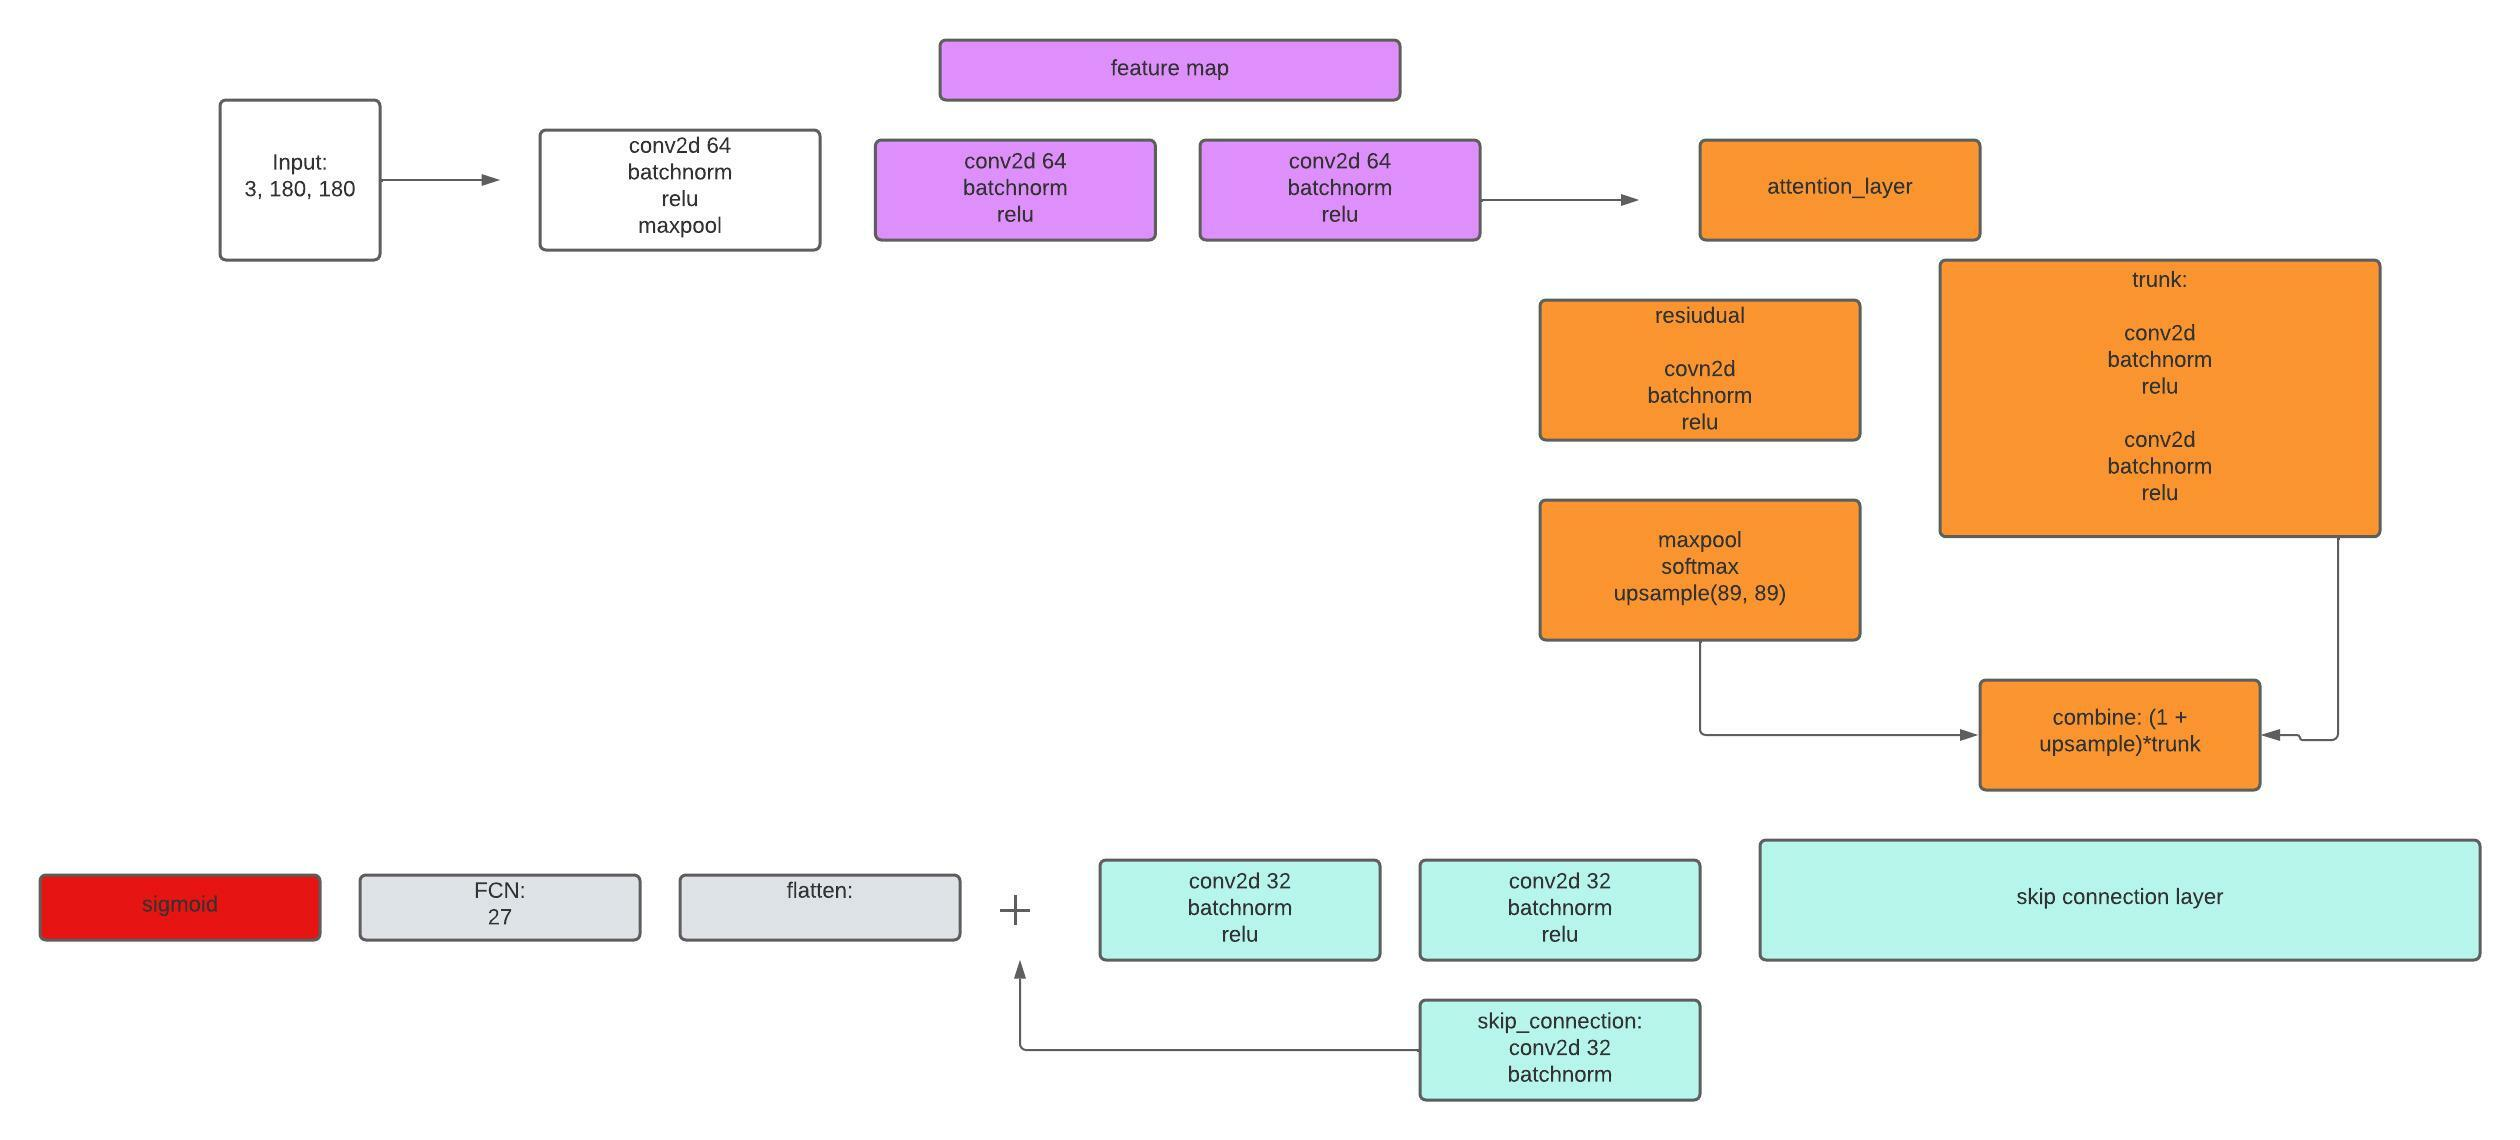
\includegraphics[width=1\textwidth]{attention_uml_v1.jpeg}
    \caption{Attention UML Diagram}
    \label{fig:attention UML diagram}
\end{figure*}

This project explores the dataset from the Lab for Media Search of the National University of Singapore \cite{nus-url}. This dataset is much larger than the popularly available Corel \cite{corel-url} and Caltech 101 \cite{caltech-url} datasets. This dataset contains:
\begin{itemize}
\item[*] 269,648 images collected from Flickr, each image is around 24k in size;
\item[*] 81 concepts of groundtruth for evaluation and their corresponding label files;
\item[*] 64-D colour histogram, 144-D colour correlogram, 73-D edge direction histogram, 128-D wavelet texture, 225-D block-wise colour moments, and 500-D bag of words based on SIFT descriptions are six types of low-level features retrieved from these images.
\end{itemize}

The classification is multitasking, which means for each image, there is more than one label. We checked the number of images corresponding to each labels in the training set. The most is sky with 36,517; the least is map with only 33. The largest number of labels in training set are listed as in Figure \ref{Data distribution}

\begin{figure} [H]
    \centering
    \includegraphics[width=0.5\textwidth]{table1_data_distribution.PNG}
    \caption{Data distribution table}
    \label{Data distribution}
\end{figure}

In addition we generated a matrix of $81*81$ to examine the relevance of the labels, as shown in Appendix \ref{labels-matrix}. 

\section{Methodology}
%Explain clearly the technical methodology, the models and algorithms that are used.  Approaches that were covered in the lectures can be described briefly, but if you are using modifications to such approaches make sure these are clearly described.    Again use citations to the literature.

%If you present algorithms, you can use the \verb+algorithm+ and \verb+algorithmic+ environments to format pseudocode (for instance, Algorithm~\ref{alg:example}). These require the corresponding style files, \verb+algorithm.sty+ and \verb+algorithmic.sty+ which are supplied with this package. 

%\begin{algorithm}[ht]
%\begin{algorithmic}
%   \STATE {\bfseries Input:} data $x_i$, size $m$
%   \REPEAT
%   \STATE Initialize $noChange = true$.
%   \FOR{$i=1$ {\bfseries to} $m-1$}
%   \IF{$x_i > x_{i+1}$} 
%   \STATE Swap $x_i$ and $x_{i+1}$
%   \STATE $noChange = false$
%   \ENDIF
%   \ENDFOR
%   \UNTIL{$noChange$ is $true$}
%\end{algorithmic}
%  \caption{Bubble Sort}
%  \label{alg:example}
%\end{algorithm}

\subsection{Model Overview}
The model combines the research into image captioning completed in the Show, Attend and Tell paper with standard strategies for multi-label classification \cite{xu2016show}. The model first passes the 3 dimensional RGB channel through a convolutional block with an RELU activation. To support identification of the rotation invariant features max pooling is used to identify the most prominent image patches. From here a basic block is utilized for more feature segmentation which consists of 2 convolutional layers, activated by RELU functions. 
\newline
\newline
Following this initial feature extraction the data is passed through an attention layer. The key features of the data are identified by passing a further convolutions block through a maxpooling. This is then activated by a Softmax function to identify the relationship, or dependencies between the image features \cite{wang2017residual}. In parallel to this attention mechanism the data is fed through 2 convolutions blocks with the output of the attention layer being: $(1 + SMAX(X))*CONV(X)$. The output of this attention block is a vector that has captured both the principal features of an image and the relationship between the features. 
\newline
\newline
The attention block is fed through a residual block where the convolution space is reduced from 64 to 32 channels. The residual layer helps to reduce the likelihood of vanishing gradient and ensure important information is propagated through to the final activation layer. As the model (as it stands) is 32 layers strategies to reduce the likelihood of vanishing/exploding gradient are appropriate. The reduction of feature layers is completed to capture non-linear relationships between the features and the labels. The final steps are creating a flat, 27 dimensional vector that is activated using the Sigmoid function. Sigmoid is chosen as an activation function because we're trying to capture the independent probability of each independent label, so is an appropriate activation function for binary-cross entropy which is used to determine the efficacy of the model.
\newline
\newline
Figure \ref{fig:attention UML diagram} contains a diagram of the model, and a full summary is included in Appendix \ref{labels-matrix}
\newline

\begin{figure*} [htp]
    \centering
    \includegraphics[width=1\textwidth]{model_summary.png}
    \caption{Model Summary}
    \label{fig:model summary}
\end{figure*}


\section{Experiments}
\label{sec:expts}
%The interim report should include some experimental results.  In most cases these will be baseline experiments.  Baseline experiments refer to experiments conducted using well-understood approaches against which you can compare later results.  For example if you were exploring a new data set, the baselines might include linear networks and deep neural networks with different numbers of hidden layers;  if you were exploring a different approach to regularisation, then the baselines would include no regularisation, and conventional techniques such as L1, L2, and dropout.  You can include the results of any further experiments in your interim report.

%Present the experimental results clearly and concisely.  Usually a result is in comparison or contrast to a result from another approach please make sure that these comparisons/contrasts are clearly presented.  You can facilitate comparisons either using graphs with multiple curves or (if appropriate, e.g. for accuracies) a results table. You need to avoid having too many figures, poorly labelled graphs, and graphs which should be comparable but which use different axis scales. A good presentation will enable the reader to compare trends in the same graph -- each graph should summarise the results relating to a particular research (sub)question.

%There is no need to include code or specific details about the compute environment.

%As before, your experimental sections should include graphs (for instance, figure~\ref{fig:sample-graph}) and/or tables (for instance, table~\ref{tab:sample-table})\footnote{These examples were taken from the ICML template paper.}, using the \verb+figure+ and \verb+table+ environments, in which you use \verb+\includegraphics+ to include an image (pdf, png, or jpg formats).  Please export graphs as 
%\href{https://en.wikipedia.org/wiki/Vector_graphics}{vector graphics}
%rather than \href{https://en.wikipedia.org/wiki/Raster_graphics}{raster
%files} as this will make sure all detail in the plot is visible.
%Matplotlib supports saving high quality figures in a wide range of
%common image formats using the
%\href{http://matplotlib.org/api/pyplot_api.html\#matplotlib.pyplot.savefig}{\texttt{savefig}}
%function. \textbf{You should use \texttt{savefig} rather than copying
%the screen-resolution raster images outputted in the notebook.} An
%example of using \texttt{savefig} to save a figure as a PDF file (which
%can be included as graphics in a \LaTeX document is given in the coursework document.

%If you need a figure or table to stretch across two columns use the \verb+figure*+ or \verb+table*+ environment instead of the \verb+figure+ or \verb+table+ environment.  Use the \verb+subfigure+ environment if you want to include multiple graphics in a single figure.

%\begin{figure}[tb]
%\vskip 5mm
%\begin{center}
%\centerline{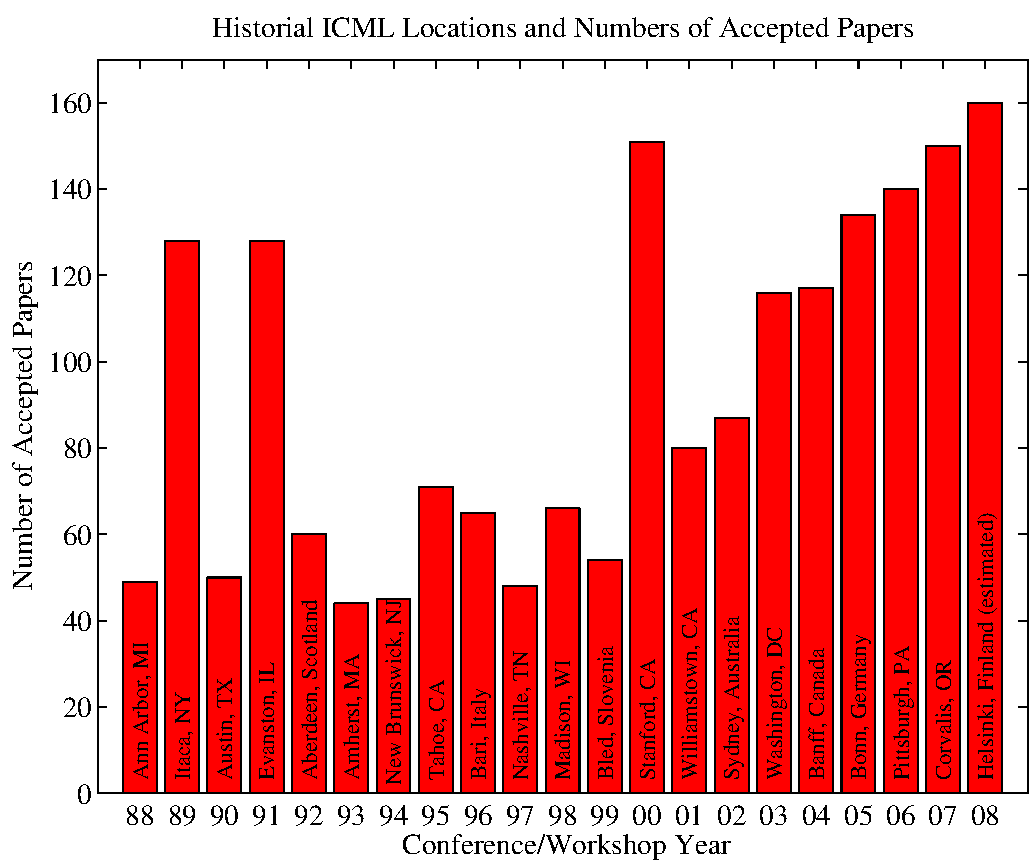
\includegraphics[width=\columnwidth]{icml_numpapers}}
%\caption{Historical locations and number of accepted papers for International
%  Machine Learning Conferences (ICML 1993 -- ICML 2008) and
%  International Workshops on Machine Learning (ML 1988 -- ML
%  1992). At the time this figure was produced, the number of
%  accepted papers for ICML 2008 was unknown and instead estimated.}
%\label{fig:sample-graph}
%\end{center}
%\vskip -5mm
%\end{figure} 

%\begin{table}[tb]
%\vskip 3mm
%\begin{center}
%\begin{small}
%\begin{sc}
%\begin{tabular}{lcccr}
%\hline
%\abovespace\belowspace
%Data set & Naive & Flexible & Better? \\
%\hline
%\abovespace
%Breast    & 95.9$\pm$ 0.2& 96.7$\pm$ 0.2& $\surd$ \\
%Cleveland & 83.3$\pm$ 0.6& 80.0$\pm$ 0.6& $\times$\\
%Glass2    & 61.9$\pm$ 1.4& 83.8$\pm$ 0.7& $\surd$ \\
%Credit    & 74.8$\pm$ 0.5& 78.3$\pm$ 0.6&         \\
%Horse     & 73.3$\pm$ 0.9& 69.7$\pm$ 1.0& $\times$\\
%Meta      & 67.1$\pm$ 0.6& 76.5$\pm$ 0.5& $\surd$ \\
%Pima      & 75.1$\pm$ 0.6& 73.9$\pm$ 0.5&         \\
%\belowspace
%Vehicle   & 44.9$\pm$ 0.6& 61.5$\pm$ 0.4& $\surd$ \\
%\hline
%\end{tabular}
%\end{sc}
%\end{small}
%\caption{Classification accuracies for naive Bayes and flexible 
%Bayes on various data sets.}
%\label{tab:sample-table}
%\end{center}
%\vskip -3mm
%\end{table}

The model was trained (initially) on a small subset of the training data. The training dataset was iterated over 35 times with back-propagation ran to support identification of model parameters to minimize the associated error with each label. 
\newline
\newline
The mean precision, error, F1 and binary cross-entropy are plotted in the figures below. The divergence in performance between the training and test dataset is typical of overfitting, where the model identifies parameters that reflect biases in the training dataset that do not extend to the overall population. 

\newline
\newline
The mean error, accuracy (both in terms of precision and recall) are plotted in the figures below. The fast convergence demonstrate that the attention model, as it stands, has a high propensity to overfit the data (no evaluation has been completed of the test dataset as of yet). To address this strategies to reduce over-fitting such as dropout and regularization will be implemented to support generalization to the test dataset. As part of improving the performance of the model we will also look at data augmentation and under what combination of labels the model performs well to develop a data augmentation strategy to address data imbalance and distribution issues. Finally, we will compare running the model with and without the attention model to explore what role it's playing in the model performance and look at visualizing the components/features identified by the attention module to see if it's aligned with the capabilities identified in the show, attend and tell paper. 

\begin{figure} [ht]
    \centering
    \includegraphics[width=0.5\textwidth]{results_small_v1_part1.png}
    \caption{BCE and recall score results}
    \label{fig:results1}
\end{figure}
\begin{figure} [ht]
    \centering
    \includegraphics[width=0.5\textwidth]{results_small_v1_part2.png}
    \caption{Precision score and F1 score results}
    \label{fig:results2}
\end{figure}


\section{Interim conclusions}
\label{sec:concl}
%What have you learned so far?  Do the experiments indicate that the project is feasible?  Do the experiments indicate that you should consider changes to your original plan?  Can you compare your results so far to what has been reported in the literature?

We used the attention model to train the NUS dataset, which contains the network images and their corresponding 81 labels in total. The difficulty in this problem lies in multitasking, e.g. an image corresponding to both the label sky cloud etc. We have currently used a small part of the dataset and have experienced overfitting. In the next step, we will expand the use of the dataset and add algorithms such as dropout to solve the overfitting. In addition, we will further investigate the issue of label correlation in the dataset to develop a better way to fit the dataset.


\section{Plan}
We would adopt the recurrent attention CNN approach\cite{fu2017look}, i.e. introduce an attention mechanism in machine learning to improve the accuracy of multi-tasking in network learning by recursively analysing local information and thus extracting the necessary features.
\label{sec:plan}
%Based on what you have done so far, present a plan for the rest of the project.  Are there any changes to the objectives?  What are the risks?  Do you need a backup plan?

%%• Plan for the remainder of the project, including discussion of risks, backup plans


\bibliography{example-refs}
 

%%\usepackage{appendix}

\begin{appendix}
% Please add the following required packages to your document preamble:
% \usepackage{graphicx}
% \usepackage{lscape}
\begin{landscape}
\begin{table}[]
\resizebox{\textwidth}{!}{%
\begin{tabular}{clllllllllllllllllllllllllllllllllllllllllllllllllllllllllllllllllllllllllllllllll}
\multicolumn{1}{l}{} &
  \multicolumn{1}{c}{\textbf{airport}} &
  \multicolumn{1}{c}{\textbf{animal}} &
  \multicolumn{1}{c}{\textbf{beach}} &
  \multicolumn{1}{c}{\textbf{bear}} &
  \multicolumn{1}{c}{\textbf{birds}} &
  \multicolumn{1}{c}{\textbf{boats}} &
  \multicolumn{1}{c}{\textbf{book}} &
  \multicolumn{1}{c}{\textbf{bridge}} &
  \multicolumn{1}{c}{\textbf{buildings}} &
  \multicolumn{1}{c}{\textbf{cars}} &
  \multicolumn{1}{c}{\textbf{castle}} &
  \multicolumn{1}{c}{\textbf{cat}} &
  \multicolumn{1}{c}{\textbf{cityscape}} &
  \multicolumn{1}{c}{\textbf{clouds}} &
  \multicolumn{1}{c}{\textbf{computer}} &
  \multicolumn{1}{c}{\textbf{coral}} &
  \multicolumn{1}{c}{\textbf{cow}} &
  \multicolumn{1}{c}{\textbf{dancing}} &
  \multicolumn{1}{c}{\textbf{dog}} &
  \multicolumn{1}{c}{\textbf{earthquake}} &
  \multicolumn{1}{c}{\textbf{elk}} &
  \multicolumn{1}{c}{\textbf{fire}} &
  \multicolumn{1}{c}{\textbf{fish}} &
  \multicolumn{1}{c}{\textbf{flags}} &
  \multicolumn{1}{c}{\textbf{flowers}} &
  \multicolumn{1}{c}{\textbf{food}} &
  \multicolumn{1}{c}{\textbf{fox}} &
  \multicolumn{1}{c}{\textbf{frost}} &
  \multicolumn{1}{c}{\textbf{garden}} &
  \multicolumn{1}{c}{\textbf{glacier}} &
  \multicolumn{1}{c}{\textbf{grass}} &
  \multicolumn{1}{c}{\textbf{harbor}} &
  \multicolumn{1}{c}{\textbf{horses}} &
  \multicolumn{1}{c}{\textbf{house}} &
  \multicolumn{1}{c}{\textbf{lake}} &
  \multicolumn{1}{c}{\textbf{leaf}} &
  \multicolumn{1}{c}{\textbf{map}} &
  \multicolumn{1}{c}{\textbf{military}} &
  \multicolumn{1}{c}{\textbf{moon}} &
  \multicolumn{1}{c}{\textbf{mountain}} &
  \multicolumn{1}{c}{\textbf{nighttime}} &
  \multicolumn{1}{c}{\textbf{ocean}} &
  \multicolumn{1}{c}{\textbf{person}} &
  \multicolumn{1}{c}{\textbf{plane}} &
  \multicolumn{1}{c}{\textbf{plants}} &
  \multicolumn{1}{c}{\textbf{police}} &
  \multicolumn{1}{c}{\textbf{protest}} &
  \multicolumn{1}{c}{\textbf{railroad}} &
  \multicolumn{1}{c}{\textbf{rainbow}} &
  \multicolumn{1}{c}{\textbf{reflection}} &
  \multicolumn{1}{c}{\textbf{road}} &
  \multicolumn{1}{c}{\textbf{rocks}} &
  \multicolumn{1}{c}{\textbf{running}} &
  \multicolumn{1}{c}{\textbf{sand}} &
  \multicolumn{1}{c}{\textbf{sign}} &
  \multicolumn{1}{c}{\textbf{sky}} &
  \multicolumn{1}{c}{\textbf{snow}} &
  \multicolumn{1}{c}{\textbf{soccer}} &
  \multicolumn{1}{c}{\textbf{sports}} &
  \multicolumn{1}{c}{\textbf{statue}} &
  \multicolumn{1}{c}{\textbf{street}} &
  \multicolumn{1}{c}{\textbf{sun}} &
  \multicolumn{1}{c}{\textbf{sunset}} &
  \multicolumn{1}{c}{\textbf{surf}} &
  \multicolumn{1}{c}{\textbf{swimmers}} &
  \multicolumn{1}{c}{\textbf{tattoo}} &
  \multicolumn{1}{c}{\textbf{temple}} &
  \multicolumn{1}{c}{\textbf{tiger}} &
  \multicolumn{1}{c}{\textbf{tower}} &
  \multicolumn{1}{c}{\textbf{town}} &
  \multicolumn{1}{c}{\textbf{toy}} &
  \multicolumn{1}{c}{\textbf{train}} &
  \multicolumn{1}{c}{\textbf{tree}} &
  \multicolumn{1}{c}{\textbf{valley}} &
  \multicolumn{1}{c}{\textbf{vehicle}} &
  \multicolumn{1}{c}{\textbf{water}} &
  \multicolumn{1}{c}{\textbf{waterfall}} &
  \multicolumn{1}{c}{\textbf{wedding}} &
  \multicolumn{1}{c}{\textbf{whales}} &
  \multicolumn{1}{c}{\textbf{window}} &
  \multicolumn{1}{c}{\textbf{zebra}} \\
\textbf{airport} &
  443 &
  443 &
  443 &
  443 &
  443 &
  443 &
  443 &
  443 &
  463 &
  463 &
  463 &
  463 &
  463 &
  729 &
  729 &
  729 &
  729 &
  729 &
  729 &
  729 &
  729 &
  729 &
  729 &
  729 &
  729 &
  729 &
  729 &
  729 &
  729 &
  729 &
  784 &
  784 &
  784 &
  785 &
  787 &
  787 &
  787 &
  905 &
  906 &
  908 &
  912 &
  916 &
  932 &
  1273 &
  1275 &
  1278 &
  1278 &
  1278 &
  1280 &
  1281 &
  1382 &
  1383 &
  1383 &
  1385 &
  1385 &
  1691 &
  1698 &
  1698 &
  1698 &
  1698 &
  1698 &
  1702 &
  1717 &
  1717 &
  1717 &
  1717 &
  1717 &
  1717 &
  1720 &
  1720 &
  1720 &
  1720 &
  1720 &
  1723 &
  1869 &
  1883 &
  1883 &
  1883 &
  1883 &
  1960 &
  1962 \\
\textbf{animal} &
  0 &
  17141 &
  17357 &
  17942 &
  19685 &
  19703 &
  19704 &
  19708 &
  19773 &
  19779 &
  19783 &
  20886 &
  20887 &
  22228 &
  22238 &
  22741 &
  23117 &
  23120 &
  24225 &
  24226 &
  24635 &
  24639 &
  25344 &
  25346 &
  25698 &
  25712 &
  25976 &
  26059 &
  26116 &
  26121 &
  28847 &
  28848 &
  29611 &
  29642 &
  29921 &
  30118 &
  30118 &
  30124 &
  30141 &
  30240 &
  30263 &
  30814 &
  31473 &
  31476 &
  31815 &
  31831 &
  31832 &
  31833 &
  31837 &
  32002 &
  32184 &
  32322 &
  32423 &
  32617 &
  32622 &
  34689 &
  35000 &
  35000 &
  35023 &
  35033 &
  35046 &
  35108 &
  35267 &
  35270 &
  35275 &
  35275 &
  35279 &
  35616 &
  35616 &
  35624 &
  35670 &
  35670 &
  35735 &
  35803 &
  35821 &
  37610 &
  37612 &
  37626 &
  37798 &
  37899 &
  38048 \\
\textbf{beach} &
  0 &
  0 &
  2588 &
  2588 &
  2622 &
  2762 &
  2762 &
  2790 &
  2861 &
  2861 &
  2864 &
  2866 &
  2871 &
  4484 &
  4484 &
  4507 &
  4511 &
  4514 &
  4554 &
  4554 &
  4554 &
  4560 &
  4565 &
  4565 &
  4571 &
  4571 &
  4572 &
  4572 &
  4575 &
  4576 &
  4662 &
  4665 &
  4671 &
  4692 &
  5582 &
  5587 &
  5587 &
  5593 &
  5601 &
  5673 &
  5696 &
  7005 &
  7354 &
  7359 &
  7408 &
  7408 &
  7408 &
  7408 &
  7416 &
  7642 &
  7675 &
  8042 &
  8054 &
  8287 &
  8291 &
  10214 &
  10246 &
  10246 &
  10258 &
  10261 &
  10261 &
  10439 &
  10874 &
  10877 &
  10892 &
  10893 &
  10895 &
  10895 &
  10904 &
  10909 &
  10912 &
  10912 &
  10949 &
  11002 &
  11025 &
  12924 &
  12924 &
  12943 &
  12943 &
  12956 &
  12956 \\
\textbf{bear} &
  0 &
  0 &
  0 &
  651 &
  651 &
  651 &
  652 &
  652 &
  652 &
  652 &
  652 &
  654 &
  654 &
  664 &
  664 &
  665 &
  665 &
  665 &
  666 &
  666 &
  668 &
  668 &
  669 &
  669 &
  670 &
  673 &
  674 &
  677 &
  677 &
  678 &
  772 &
  772 &
  772 &
  772 &
  774 &
  786 &
  786 &
  786 &
  786 &
  786 &
  786 &
  794 &
  808 &
  808 &
  817 &
  817 &
  817 &
  817 &
  817 &
  820 &
  828 &
  834 &
  834 &
  834 &
  834 &
  849 &
  866 &
  866 &
  866 &
  866 &
  866 &
  866 &
  866 &
  866 &
  866 &
  866 &
  866 &
  866 &
  866 &
  866 &
  883 &
  883 &
  883 &
  883 &
  883 &
  983 &
  983 &
  984 &
  984 &
  984 &
  984 \\
\textbf{birds} &
  0 &
  0 &
  0 &
  0 &
  1905 &
  1906 &
  1906 &
  1908 &
  1917 &
  1917 &
  1919 &
  1921 &
  1921 &
  2215 &
  2215 &
  2217 &
  2217 &
  2218 &
  2219 &
  2219 &
  2219 &
  2219 &
  2229 &
  2229 &
  2253 &
  2254 &
  2257 &
  2264 &
  2272 &
  2272 &
  2396 &
  2396 &
  2396 &
  2397 &
  2468 &
  2492 &
  2492 &
  2492 &
  2499 &
  2502 &
  2504 &
  2569 &
  2589 &
  2590 &
  2613 &
  2613 &
  2613 &
  2613 &
  2613 &
  2653 &
  2666 &
  2684 &
  2685 &
  2690 &
  2690 &
  3101 &
  3116 &
  3116 &
  3116 &
  3118 &
  3118 &
  3127 &
  3157 &
  3157 &
  3157 &
  3157 &
  3157 &
  3157 &
  3157 &
  3158 &
  3163 &
  3163 &
  3165 &
  3168 &
  3169 &
  3440 &
  3440 &
  3441 &
  3441 &
  3447 &
  3447 \\
\textbf{boats} &
  0 &
  0 &
  0 &
  0 &
  0 &
  2057 &
  2057 &
  2110 &
  2398 &
  2398 &
  2398 &
  2398 &
  2448 &
  3506 &
  3506 &
  3510 &
  3510 &
  3510 &
  3512 &
  3512 &
  3512 &
  3512 &
  3514 &
  3517 &
  3519 &
  3519 &
  3520 &
  3521 &
  3529 &
  3530 &
  3571 &
  3718 &
  3718 &
  3781 &
  4467 &
  4471 &
  4471 &
  4499 &
  4502 &
  4545 &
  4607 &
  5193 &
  5287 &
  5290 &
  5312 &
  5319 &
  5319 &
  5320 &
  5322 &
  5789 &
  5799 &
  5844 &
  5844 &
  5862 &
  5863 &
  7272 &
  7294 &
  7294 &
  7298 &
  7298 &
  7303 &
  7381 &
  7601 &
  7602 &
  7602 &
  7602 &
  7604 &
  7604 &
  7622 &
  7687 &
  7694 &
  7697 &
  7710 &
  7744 &
  8048 &
  9573 &
  9573 &
  9577 &
  9580 &
  9747 &
  9747 \\
\textbf{book} &
  0 &
  0 &
  0 &
  0 &
  0 &
  0 &
  157 &
  157 &
  158 &
  158 &
  158 &
  158 &
  158 &
  159 &
  162 &
  162 &
  162 &
  162 &
  163 &
  163 &
  163 &
  163 &
  163 &
  163 &
  164 &
  164 &
  164 &
  164 &
  164 &
  164 &
  165 &
  165 &
  165 &
  165 &
  165 &
  165 &
  165 &
  165 &
  165 &
  165 &
  165 &
  165 &
  173 &
  173 &
  173 &
  173 &
  173 &
  173 &
  173 &
  173 &
  173 &
  173 &
  173 &
  173 &
  173 &
  176 &
  176 &
  176 &
  176 &
  176 &
  176 &
  176 &
  176 &
  176 &
  176 &
  176 &
  176 &
  176 &
  177 &
  177 &
  183 &
  183 &
  183 &
  183 &
  183 &
  183 &
  183 &
  183 &
  183 &
  186 &
  186 \\
\textbf{bridge} &
  0 &
  0 &
  0 &
  0 &
  0 &
  0 &
  0 &
  1170 &
  1383 &
  1387 &
  1393 &
  1393 &
  1473 &
  2009 &
  2009 &
  2010 &
  2010 &
  2010 &
  2010 &
  2010 &
  2010 &
  2014 &
  2014 &
  2015 &
  2021 &
  2021 &
  2021 &
  2027 &
  2064 &
  2064 &
  2151 &
  2162 &
  2162 &
  2177 &
  2374 &
  2376 &
  2376 &
  2380 &
  2390 &
  2406 &
  2532 &
  2641 &
  2672 &
  2674 &
  2711 &
  2713 &
  2714 &
  2759 &
  2759 &
  2936 &
  3036 &
  3073 &
  3074 &
  3077 &
  3078 &
  3746 &
  3767 &
  3767 &
  3767 &
  3768 &
  3774 &
  3804 &
  3887 &
  3887 &
  3887 &
  3887 &
  3887 &
  3887 &
  3925 &
  3950 &
  3951 &
  3972 &
  3982 &
  3991 &
  4008 &
  4524 &
  4527 &
  4529 &
  4529 &
  4564 &
  4564 \\
\textbf{buildings} &
  0 &
  0 &
  0 &
  0 &
  0 &
  0 &
  0 &
  0 &
  8732 &
  8800 &
  8945 &
  8951 &
  9808 &
  13417 &
  13419 &
  13425 &
  13426 &
  13427 &
  13438 &
  13442 &
  13443 &
  13469 &
  13469 &
  13487 &
  13524 &
  13524 &
  13528 &
  13548 &
  13747 &
  13747 &
  14410 &
  14487 &
  14498 &
  15330 &
  15850 &
  15856 &
  15856 &
  15891 &
  15940 &
  16044 &
  16837 &
  17017 &
  17566 &
  17595 &
  17807 &
  17866 &
  17899 &
  17925 &
  17949 &
  18603 &
  19245 &
  19336 &
  19340 &
  19359 &
  19427 &
  24608 &
  24782 &
  24782 &
  24785 &
  24822 &
  25270 &
  25329 &
  25617 &
  25617 &
  25618 &
  25619 &
  25872 &
  25872 &
  26388 &
  27110 &
  27129 &
  27147 &
  27248 &
  27324 &
  27601 &
  28988 &
  28988 &
  28999 &
  28999 &
  31180 &
  31181 \\
\textbf{cars} &
  0 &
  0 &
  0 &
  0 &
  0 &
  0 &
  0 &
  0 &
  0 &
  763 &
  763 &
  763 &
  766 &
  908 &
  908 &
  908 &
  908 &
  908 &
  914 &
  914 &
  915 &
  918 &
  918 &
  919 &
  919 &
  919 &
  919 &
  921 &
  923 &
  923 &
  984 &
  984 &
  985 &
  993 &
  996 &
  996 &
  996 &
  1000 &
  1000 &
  1005 &
  1024 &
  1027 &
  1116 &
  1117 &
  1130 &
  1157 &
  1157 &
  1193 &
  1193 &
  1195 &
  1440 &
  1441 &
  1441 &
  1448 &
  1449 &
  1661 &
  1682 &
  1682 &
  1693 &
  1693 &
  1742 &
  1745 &
  1755 &
  1755 &
  1755 &
  1756 &
  1757 &
  1757 &
  1761 &
  1782 &
  1796 &
  1853 &
  1855 &
  1859 &
  2162 &
  2175 &
  2175 &
  2178 &
  2178 &
  2472 &
  2472 \\
\textbf{castle} &
  0 &
  0 &
  0 &
  0 &
  0 &
  0 &
  0 &
  0 &
  0 &
  0 &
  266 &
  266 &
  270 &
  415 &
  415 &
  415 &
  415 &
  415 &
  415 &
  415 &
  415 &
  415 &
  415 &
  415 &
  416 &
  416 &
  416 &
  416 &
  433 &
  433 &
  481 &
  481 &
  481 &
  491 &
  506 &
  506 &
  506 &
  509 &
  509 &
  513 &
  516 &
  523 &
  527 &
  529 &
  545 &
  545 &
  546 &
  546 &
  546 &
  566 &
  569 &
  586 &
  586 &
  589 &
  589 &
  792 &
  794 &
  794 &
  795 &
  795 &
  795 &
  796 &
  801 &
  801 &
  801 &
  801 &
  817 &
  817 &
  843 &
  848 &
  848 &
  849 &
  855 &
  857 &
  860 &
  894 &
  894 &
  895 &
  895 &
  953 &
  953 \\
\textbf{cat} &
  0 &
  0 &
  0 &
  0 &
  0 &
  0 &
  0 &
  0 &
  0 &
  0 &
  0 &
  1208 &
  1208 &
  1225 &
  1231 &
  1231 &
  1231 &
  1231 &
  1247 &
  1247 &
  1247 &
  1247 &
  1248 &
  1248 &
  1256 &
  1257 &
  1261 &
  1262 &
  1266 &
  1266 &
  1365 &
  1365 &
  1367 &
  1368 &
  1369 &
  1377 &
  1377 &
  1378 &
  1378 &
  1378 &
  1379 &
  1383 &
  1413 &
  1414 &
  1421 &
  1421 &
  1421 &
  1421 &
  1421 &
  1423 &
  1431 &
  1431 &
  1433 &
  1433 &
  1433 &
  1470 &
  1475 &
  1475 &
  1475 &
  1475 &
  1478 &
  1478 &
  1478 &
  1478 &
  1478 &
  1478 &
  1480 &
  1497 &
  1497 &
  1501 &
  1507 &
  1507 &
  1508 &
  1508 &
  1508 &
  1529 &
  1529 &
  1529 &
  1529 &
  1559 &
  1560 \\
\textbf{cityscape} &
  0 &
  0 &
  0 &
  0 &
  0 &
  0 &
  0 &
  0 &
  0 &
  0 &
  0 &
  0 &
  1108 &
  1704 &
  1704 &
  1706 &
  1706 &
  1706 &
  1706 &
  1706 &
  1706 &
  1710 &
  1710 &
  1710 &
  1710 &
  1710 &
  1711 &
  1711 &
  1718 &
  1718 &
  1741 &
  1765 &
  1765 &
  1768 &
  1872 &
  1872 &
  1872 &
  1874 &
  1895 &
  1901 &
  2245 &
  2273 &
  2299 &
  2301 &
  2308 &
  2309 &
  2309 &
  2314 &
  2317 &
  2473 &
  2575 &
  2578 &
  2578 &
  2579 &
  2579 &
  3285 &
  3295 &
  3295 &
  3295 &
  3300 &
  3345 &
  3354 &
  3426 &
  3426 &
  3426 &
  3426 &
  3433 &
  3433 &
  3574 &
  3655 &
  3655 &
  3658 &
  3663 &
  3665 &
  3682 &
  3973 &
  3973 &
  3975 &
  3975 &
  4023 &
  4023 \\
\textbf{clouds} &
  0 &
  0 &
  0 &
  0 &
  0 &
  0 &
  0 &
  0 &
  0 &
  0 &
  0 &
  0 &
  0 &
  26929 &
  26932 &
  26976 &
  27097 &
  27111 &
  27168 &
  27176 &
  27201 &
  27368 &
  27381 &
  27418 &
  27684 &
  27690 &
  27700 &
  27824 &
  28124 &
  28245 &
  31948 &
  32096 &
  32229 &
  33161 &
  37430 &
  37462 &
  37462 &
  38021 &
  38242 &
  39867 &
  40476 &
  43913 &
  45430 &
  46179 &
  47890 &
  47928 &
  47941 &
  48092 &
  48232 &
  50287 &
  51569 &
  53056 &
  53070 &
  53552 &
  53662 &
  76164 &
  77131 &
  77134 &
  77215 &
  77306 &
  77476 &
  78842 &
  82209 &
  82219 &
  82248 &
  82252 &
  82556 &
  82557 &
  83288 &
  83624 &
  83696 &
  83831 &
  84835 &
  86109 &
  86952 &
  94763 &
  94775 &
  94859 &
  94883 &
  96338 &
  96342 \\
\textbf{computer} &
  0 &
  0 &
  0 &
  0 &
  0 &
  0 &
  0 &
  0 &
  0 &
  0 &
  0 &
  0 &
  0 &
  0 &
  246 &
  246 &
  246 &
  246 &
  247 &
  247 &
  247 &
  247 &
  247 &
  247 &
  249 &
  249 &
  249 &
  249 &
  249 &
  249 &
  250 &
  250 &
  251 &
  251 &
  251 &
  251 &
  251 &
  251 &
  251 &
  252 &
  253 &
  253 &
  304 &
  304 &
  305 &
  305 &
  305 &
  305 &
  305 &
  305 &
  307 &
  307 &
  307 &
  308 &
  308 &
  316 &
  316 &
  316 &
  316 &
  316 &
  316 &
  316 &
  316 &
  316 &
  316 &
  316 &
  316 &
  316 &
  316 &
  316 &
  318 &
  318 &
  318 &
  318 &
  318 &
  318 &
  318 &
  318 &
  318 &
  331 &
  331 \\
\textbf{coral} &
  0 &
  0 &
  0 &
  0 &
  0 &
  0 &
  0 &
  0 &
  0 &
  0 &
  0 &
  0 &
  0 &
  0 &
  0 &
  841 &
  841 &
  841 &
  842 &
  842 &
  843 &
  843 &
  1256 &
  1256 &
  1284 &
  1285 &
  1285 &
  1287 &
  1289 &
  1289 &
  1298 &
  1298 &
  1298 &
  1299 &
  1343 &
  1347 &
  1347 &
  1347 &
  1347 &
  1348 &
  1353 &
  1581 &
  1606 &
  1606 &
  1619 &
  1619 &
  1619 &
  1619 &
  1619 &
  1626 &
  1630 &
  1644 &
  1645 &
  1649 &
  1649 &
  1719 &
  1719 &
  1719 &
  1720 &
  1721 &
  1721 &
  1724 &
  1735 &
  1738 &
  1753 &
  1753 &
  1753 &
  1753 &
  1754 &
  1754 &
  1754 &
  1754 &
  1756 &
  1760 &
  1760 &
  2231 &
  2231 &
  2231 &
  2249 &
  2251 &
  2251 \\
\textbf{cow} &
  0 &
  0 &
  0 &
  0 &
  0 &
  0 &
  0 &
  0 &
  0 &
  0 &
  0 &
  0 &
  0 &
  0 &
  0 &
  0 &
  398 &
  398 &
  402 &
  402 &
  412 &
  413 &
  413 &
  413 &
  418 &
  418 &
  418 &
  418 &
  419 &
  419 &
  636 &
  636 &
  647 &
  647 &
  656 &
  660 &
  660 &
  660 &
  660 &
  670 &
  670 &
  674 &
  687 &
  687 &
  700 &
  701 &
  701 &
  701 &
  701 &
  712 &
  716 &
  719 &
  720 &
  727 &
  727 &
  880 &
  886 &
  886 &
  886 &
  886 &
  886 &
  887 &
  896 &
  896 &
  896 &
  896 &
  896 &
  896 &
  896 &
  896 &
  896 &
  896 &
  904 &
  916 &
  916 &
  938 &
  938 &
  938 &
  938 &
  938 &
  938 \\
\textbf{dancing} &
  0 &
  0 &
  0 &
  0 &
  0 &
  0 &
  0 &
  0 &
  0 &
  0 &
  0 &
  0 &
  0 &
  0 &
  0 &
  0 &
  0 &
  393 &
  394 &
  394 &
  394 &
  398 &
  398 &
  398 &
  398 &
  398 &
  398 &
  398 &
  399 &
  399 &
  421 &
  421 &
  421 &
  421 &
  425 &
  425 &
  425 &
  425 &
  425 &
  426 &
  428 &
  433 &
  721 &
  721 &
  723 &
  723 &
  723 &
  723 &
  723 &
  723 &
  727 &
  729 &
  729 &
  730 &
  730 &
  758 &
  759 &
  759 &
  782 &
  782 &
  783 &
  786 &
  792 &
  792 &
  792 &
  793 &
  793 &
  793 &
  793 &
  793 &
  794 &
  794 &
  794 &
  796 &
  797 &
  810 &
  810 &
  820 &
  820 &
  824 &
  824 \\
\textbf{dog} &
  0 &
  0 &
  0 &
  0 &
  0 &
  0 &
  0 &
  0 &
  0 &
  0 &
  0 &
  0 &
  0 &
  0 &
  0 &
  0 &
  0 &
  0 &
  1222 &
  1222 &
  1222 &
  1223 &
  1224 &
  1225 &
  1237 &
  1237 &
  1246 &
  1249 &
  1258 &
  1258 &
  1458 &
  1458 &
  1458 &
  1463 &
  1484 &
  1492 &
  1492 &
  1492 &
  1493 &
  1499 &
  1500 &
  1518 &
  1606 &
  1606 &
  1617 &
  1617 &
  1617 &
  1618 &
  1618 &
  1631 &
  1651 &
  1654 &
  1689 &
  1695 &
  1695 &
  1796 &
  1837 &
  1837 &
  1837 &
  1837 &
  1841 &
  1843 &
  1847 &
  1847 &
  1847 &
  1847 &
  1848 &
  1849 &
  1849 &
  1849 &
  1867 &
  1867 &
  1868 &
  1868 &
  1875 &
  1955 &
  1955 &
  1959 &
  1959 &
  1980 &
  1980 \\
\textbf{earthquake} &
  0 &
  0 &
  0 &
  0 &
  0 &
  0 &
  0 &
  0 &
  0 &
  0 &
  0 &
  0 &
  0 &
  0 &
  0 &
  0 &
  0 &
  0 &
  0 &
  36 &
  36 &
  36 &
  36 &
  36 &
  36 &
  36 &
  36 &
  36 &
  36 &
  36 &
  37 &
  37 &
  37 &
  39 &
  39 &
  39 &
  39 &
  39 &
  39 &
  39 &
  39 &
  39 &
  53 &
  53 &
  53 &
  54 &
  54 &
  54 &
  54 &
  54 &
  54 &
  55 &
  55 &
  56 &
  56 &
  67 &
  67 &
  67 &
  67 &
  67 &
  67 &
  68 &
  68 &
  68 &
  68 &
  68 &
  68 &
  68 &
  68 &
  68 &
  68 &
  68 &
  68 &
  68 &
  68 &
  68 &
  68 &
  68 &
  68 &
  72 &
  72 \\
\textbf{elk} &
  0 &
  0 &
  0 &
  0 &
  0 &
  0 &
  0 &
  0 &
  0 &
  0 &
  0 &
  0 &
  0 &
  0 &
  0 &
  0 &
  0 &
  0 &
  0 &
  0 &
  419 &
  421 &
  421 &
  421 &
  421 &
  421 &
  423 &
  437 &
  438 &
  438 &
  641 &
  641 &
  642 &
  642 &
  651 &
  658 &
  658 &
  658 &
  659 &
  666 &
  666 &
  666 &
  670 &
  670 &
  699 &
  700 &
  700 &
  700 &
  700 &
  704 &
  706 &
  710 &
  713 &
  715 &
  716 &
  761 &
  793 &
  793 &
  793 &
  793 &
  793 &
  793 &
  797 &
  797 &
  797 &
  797 &
  797 &
  797 &
  797 &
  797 &
  797 &
  797 &
  799 &
  802 &
  803 &
  825 &
  825 &
  825 &
  825 &
  825 &
  825 \\
\textbf{fire} &
  0 &
  0 &
  0 &
  0 &
  0 &
  0 &
  0 &
  0 &
  0 &
  0 &
  0 &
  0 &
  0 &
  0 &
  0 &
  0 &
  0 &
  0 &
  0 &
  0 &
  0 &
  548 &
  548 &
  548 &
  549 &
  551 &
  551 &
  551 &
  552 &
  552 &
  568 &
  568 &
  569 &
  575 &
  597 &
  597 &
  597 &
  614 &
  619 &
  626 &
  682 &
  697 &
  799 &
  816 &
  826 &
  834 &
  834 &
  835 &
  837 &
  852 &
  877 &
  881 &
  881 &
  883 &
  883 &
  1097 &
  1098 &
  1098 &
  1100 &
  1100 &
  1102 &
  1119 &
  1157 &
  1157 &
  1157 &
  1157 &
  1158 &
  1158 &
  1165 &
  1168 &
  1170 &
  1170 &
  1175 &
  1179 &
  1186 &
  1238 &
  1238 &
  1241 &
  1241 &
  1260 &
  1260 \\
\textbf{fish} &
  0 &
  0 &
  0 &
  0 &
  0 &
  0 &
  0 &
  0 &
  0 &
  0 &
  0 &
  0 &
  0 &
  0 &
  0 &
  0 &
  0 &
  0 &
  0 &
  0 &
  0 &
  0 &
  873 &
  873 &
  882 &
  885 &
  885 &
  886 &
  890 &
  890 &
  899 &
  899 &
  899 &
  899 &
  915 &
  916 &
  916 &
  916 &
  916 &
  916 &
  918 &
  1099 &
  1127 &
  1127 &
  1130 &
  1130 &
  1130 &
  1130 &
  1130 &
  1134 &
  1138 &
  1143 &
  1143 &
  1145 &
  1145 &
  1176 &
  1177 &
  1177 &
  1178 &
  1179 &
  1179 &
  1180 &
  1181 &
  1181 &
  1186 &
  1186 &
  1186 &
  1186 &
  1186 &
  1186 &
  1186 &
  1186 &
  1186 &
  1186 &
  1186 &
  1668 &
  1668 &
  1668 &
  1695 &
  1698 &
  1698 \\
\textbf{flags} &
  0 &
  0 &
  0 &
  0 &
  0 &
  0 &
  0 &
  0 &
  0 &
  0 &
  0 &
  0 &
  0 &
  0 &
  0 &
  0 &
  0 &
  0 &
  0 &
  0 &
  0 &
  0 &
  0 &
  171 &
  171 &
  171 &
  171 &
  171 &
  172 &
  173 &
  183 &
  183 &
  183 &
  183 &
  184 &
  184 &
  184 &
  187 &
  187 &
  189 &
  190 &
  193 &
  223 &
  223 &
  223 &
  223 &
  233 &
  233 &
  233 &
  233 &
  239 &
  240 &
  240 &
  241 &
  242 &
  310 &
  312 &
  312 &
  313 &
  313 &
  315 &
  316 &
  319 &
  319 &
  319 &
  319 &
  319 &
  319 &
  321 &
  323 &
  324 &
  324 &
  324 &
  325 &
  328 &
  332 &
  332 &
  332 &
  332 &
  348 &
  348 \\
\textbf{flowers} &
  0 &
  0 &
  0 &
  0 &
  0 &
  0 &
  0 &
  0 &
  0 &
  0 &
  0 &
  0 &
  0 &
  0 &
  0 &
  0 &
  0 &
  0 &
  0 &
  0 &
  0 &
  0 &
  0 &
  0 &
  4290 &
  4299 &
  4306 &
  4320 &
  4596 &
  4597 &
  5004 &
  5004 &
  5008 &
  5032 &
  5053 &
  5270 &
  5270 &
  5270 &
  5273 &
  5290 &
  5295 &
  5307 &
  5358 &
  5358 &
  7472 &
  7472 &
  7472 &
  7473 &
  7474 &
  7512 &
  7530 &
  7546 &
  7547 &
  7547 &
  7547 &
  7980 &
  7987 &
  7987 &
  7988 &
  7990 &
  7992 &
  8010 &
  8025 &
  8025 &
  8025 &
  8025 &
  8027 &
  8027 &
  8031 &
  8041 &
  8047 &
  8048 &
  8102 &
  8119 &
  8124 &
  8298 &
  8299 &
  8314 &
  8314 &
  8369 &
  8369 \\
\textbf{food} &
  0 &
  0 &
  0 &
  0 &
  0 &
  0 &
  0 &
  0 &
  0 &
  0 &
  0 &
  0 &
  0 &
  0 &
  0 &
  0 &
  0 &
  0 &
  0 &
  0 &
  0 &
  0 &
  0 &
  0 &
  0 &
  1327 &
  1327 &
  1330 &
  1330 &
  1330 &
  1337 &
  1337 &
  1337 &
  1337 &
  1337 &
  1351 &
  1351 &
  1351 &
  1351 &
  1351 &
  1351 &
  1352 &
  1391 &
  1391 &
  1450 &
  1450 &
  1450 &
  1450 &
  1450 &
  1451 &
  1452 &
  1454 &
  1454 &
  1454 &
  1454 &
  1464 &
  1465 &
  1465 &
  1465 &
  1466 &
  1466 &
  1467 &
  1467 &
  1467 &
  1467 &
  1467 &
  1467 &
  1467 &
  1467 &
  1467 &
  1495 &
  1495 &
  1495 &
  1495 &
  1495 &
  1523 &
  1523 &
  1528 &
  1528 &
  1529 &
  1529 \\
\textbf{fox} &
  0 &
  0 &
  0 &
  0 &
  0 &
  0 &
  0 &
  0 &
  0 &
  0 &
  0 &
  0 &
  0 &
  0 &
  0 &
  0 &
  0 &
  0 &
  0 &
  0 &
  0 &
  0 &
  0 &
  0 &
  0 &
  0 &
  333 &
  335 &
  340 &
  340 &
  439 &
  439 &
  441 &
  442 &
  445 &
  449 &
  449 &
  449 &
  449 &
  450 &
  450 &
  451 &
  463 &
  463 &
  482 &
  482 &
  482 &
  482 &
  482 &
  484 &
  488 &
  494 &
  495 &
  496 &
  496 &
  512 &
  529 &
  529 &
  531 &
  532 &
  532 &
  533 &
  533 &
  533 &
  533 &
  533 &
  534 &
  534 &
  535 &
  535 &
  536 &
  536 &
  539 &
  539 &
  539 &
  545 &
  545 &
  545 &
  545 &
  546 &
  547 \\
\textbf{frost} &
  0 &
  0 &
  0 &
  0 &
  0 &
  0 &
  0 &
  0 &
  0 &
  0 &
  0 &
  0 &
  0 &
  0 &
  0 &
  0 &
  0 &
  0 &
  0 &
  0 &
  0 &
  0 &
  0 &
  0 &
  0 &
  0 &
  0 &
  565 &
  568 &
  578 &
  604 &
  604 &
  608 &
  619 &
  639 &
  653 &
  653 &
  655 &
  655 &
  670 &
  670 &
  679 &
  694 &
  694 &
  762 &
  762 &
  762 &
  765 &
  765 &
  779 &
  798 &
  816 &
  817 &
  820 &
  820 &
  1010 &
  1286 &
  1286 &
  1287 &
  1288 &
  1291 &
  1303 &
  1314 &
  1315 &
  1315 &
  1315 &
  1315 &
  1315 &
  1316 &
  1316 &
  1318 &
  1321 &
  1427 &
  1438 &
  1442 &
  1505 &
  1505 &
  1505 &
  1505 &
  1539 &
  1539 \\
\textbf{garden} &
  0 &
  0 &
  0 &
  0 &
  0 &
  0 &
  0 &
  0 &
  0 &
  0 &
  0 &
  0 &
  0 &
  0 &
  0 &
  0 &
  0 &
  0 &
  0 &
  0 &
  0 &
  0 &
  0 &
  0 &
  0 &
  0 &
  0 &
  0 &
  1487 &
  1487 &
  2287 &
  2287 &
  2292 &
  2494 &
  2585 &
  2618 &
  2618 &
  2619 &
  2620 &
  2662 &
  2671 &
  2673 &
  2725 &
  2726 &
  3209 &
  3210 &
  3210 &
  3213 &
  3216 &
  3334 &
  3388 &
  3427 &
  3427 &
  3431 &
  3431 &
  3968 &
  3978 &
  3979 &
  3979 &
  3991 &
  3994 &
  4004 &
  4029 &
  4030 &
  4030 &
  4032 &
  4059 &
  4059 &
  4071 &
  4105 &
  4108 &
  4110 &
  4296 &
  4333 &
  4343 &
  4561 &
  4566 &
  4571 &
  4571 &
  4699 &
  4699 \\
\textbf{glacier} &
  0 &
  0 &
  0 &
  0 &
  0 &
  0 &
  0 &
  0 &
  0 &
  0 &
  0 &
  0 &
  0 &
  0 &
  0 &
  0 &
  0 &
  0 &
  0 &
  0 &
  0 &
  0 &
  0 &
  0 &
  0 &
  0 &
  0 &
  0 &
  0 &
  252 &
  264 &
  264 &
  264 &
  265 &
  331 &
  332 &
  332 &
  332 &
  332 &
  468 &
  468 &
  486 &
  491 &
  491 &
  499 &
  500 &
  500 &
  500 &
  500 &
  528 &
  529 &
  624 &
  624 &
  624 &
  624 &
  793 &
  909 &
  909 &
  910 &
  910 &
  910 &
  911 &
  919 &
  919 &
  920 &
  920 &
  920 &
  920 &
  920 &
  920 &
  922 &
  922 &
  929 &
  1025 &
  1026 &
  1117 &
  1117 &
  1117 &
  1117 &
  1118 &
  1118 \\
\textbf{grass} &
  0 &
  0 &
  0 &
  0 &
  0 &
  0 &
  0 &
  0 &
  0 &
  0 &
  0 &
  0 &
  0 &
  0 &
  0 &
  0 &
  0 &
  0 &
  0 &
  0 &
  0 &
  0 &
  0 &
  0 &
  0 &
  0 &
  0 &
  0 &
  0 &
  0 &
  11176 &
  11176 &
  11488 &
  12236 &
  12762 &
  12850 &
  12850 &
  12953 &
  12968 &
  13561 &
  13593 &
  13759 &
  14798 &
  14884 &
  17065 &
  17088 &
  17094 &
  17163 &
  17216 &
  17643 &
  18201 &
  18612 &
  18666 &
  18793 &
  18829 &
  23802 &
  23878 &
  23929 &
  24083 &
  24111 &
  24125 &
  24257 &
  24565 &
  24569 &
  24569 &
  24573 &
  24620 &
  24661 &
  24715 &
  24767 &
  24801 &
  24836 &
  25595 &
  26192 &
  26465 &
  27656 &
  27677 &
  27727 &
  27728 &
  28188 &
  28212 \\
\textbf{harbor} &
  0 &
  0 &
  0 &
  0 &
  0 &
  0 &
  0 &
  0 &
  0 &
  0 &
  0 &
  0 &
  0 &
  0 &
  0 &
  0 &
  0 &
  0 &
  0 &
  0 &
  0 &
  0 &
  0 &
  0 &
  0 &
  0 &
  0 &
  0 &
  0 &
  0 &
  0 &
  247 &
  247 &
  254 &
  349 &
  349 &
  349 &
  352 &
  353 &
  358 &
  385 &
  423 &
  426 &
  426 &
  427 &
  427 &
  427 &
  427 &
  428 &
  535 &
  539 &
  541 &
  541 &
  541 &
  541 &
  741 &
  742 &
  742 &
  742 &
  742 &
  745 &
  756 &
  803 &
  803 &
  803 &
  803 &
  803 &
  803 &
  808 &
  831 &
  831 &
  831 &
  833 &
  835 &
  872 &
  1079 &
  1079 &
  1079 &
  1079 &
  1096 &
  1096 \\
\textbf{horses} &
  0 &
  0 &
  0 &
  0 &
  0 &
  0 &
  0 &
  0 &
  0 &
  0 &
  0 &
  0 &
  0 &
  0 &
  0 &
  0 &
  0 &
  0 &
  0 &
  0 &
  0 &
  0 &
  0 &
  0 &
  0 &
  0 &
  0 &
  0 &
  0 &
  0 &
  0 &
  0 &
  900 &
  906 &
  911 &
  911 &
  911 &
  915 &
  915 &
  926 &
  928 &
  932 &
  1113 &
  1113 &
  1147 &
  1161 &
  1162 &
  1162 &
  1162 &
  1165 &
  1176 &
  1180 &
  1210 &
  1232 &
  1232 &
  1487 &
  1513 &
  1513 &
  1530 &
  1530 &
  1531 &
  1538 &
  1550 &
  1550 &
  1550 &
  1550 &
  1551 &
  1551 &
  1551 &
  1551 &
  1553 &
  1553 &
  1560 &
  1567 &
  1568 &
  1595 &
  1595 &
  1595 &
  1595 &
  1607 &
  1610 \\
\textbf{house} &
  0 &
  0 &
  0 &
  0 &
  0 &
  0 &
  0 &
  0 &
  0 &
  0 &
  0 &
  0 &
  0 &
  0 &
  0 &
  0 &
  0 &
  0 &
  0 &
  0 &
  0 &
  0 &
  0 &
  0 &
  0 &
  0 &
  0 &
  0 &
  0 &
  0 &
  0 &
  0 &
  0 &
  1924 &
  2076 &
  2080 &
  2080 &
  2084 &
  2091 &
  2196 &
  2213 &
  2271 &
  2314 &
  2316 &
  2557 &
  2560 &
  2560 &
  2564 &
  2568 &
  2728 &
  2819 &
  2880 &
  2880 &
  2901 &
  2904 &
  4238 &
  4323 &
  4323 &
  4325 &
  4330 &
  4357 &
  4370 &
  4427 &
  4427 &
  4427 &
  4427 &
  4435 &
  4435 &
  4450 &
  4569 &
  4573 &
  4577 &
  4657 &
  4739 &
  4801 &
  5135 &
  5137 &
  5138 &
  5138 &
  5714 &
  5714 \\
\textbf{lake} &
  0 &
  0 &
  0 &
  0 &
  0 &
  0 &
  0 &
  0 &
  0 &
  0 &
  0 &
  0 &
  0 &
  0 &
  0 &
  0 &
  0 &
  0 &
  0 &
  0 &
  0 &
  0 &
  0 &
  0 &
  0 &
  0 &
  0 &
  0 &
  0 &
  0 &
  0 &
  0 &
  0 &
  0 &
  6715 &
  6721 &
  6721 &
  6764 &
  6795 &
  7395 &
  7543 &
  9827 &
  10148 &
  10164 &
  10536 &
  10540 &
  10540 &
  10545 &
  10568 &
  12515 &
  12613 &
  13358 &
  13359 &
  13438 &
  13440 &
  18558 &
  18784 &
  18784 &
  18799 &
  18801 &
  18805 &
  19313 &
  20638 &
  20664 &
  20679 &
  20680 &
  20710 &
  20716 &
  20774 &
  20852 &
  20866 &
  20869 &
  21079 &
  21579 &
  21762 &
  27437 &
  27477 &
  27488 &
  27536 &
  27645 &
  27645 \\
\textbf{leaf} &
  0 &
  0 &
  0 &
  0 &
  0 &
  0 &
  0 &
  0 &
  0 &
  0 &
  0 &
  0 &
  0 &
  0 &
  0 &
  0 &
  0 &
  0 &
  0 &
  0 &
  0 &
  0 &
  0 &
  0 &
  0 &
  0 &
  0 &
  0 &
  0 &
  0 &
  0 &
  0 &
  0 &
  0 &
  0 &
  899 &
  899 &
  900 &
  900 &
  903 &
  904 &
  909 &
  930 &
  930 &
  1179 &
  1179 &
  1179 &
  1179 &
  1179 &
  1185 &
  1192 &
  1202 &
  1202 &
  1202 &
  1202 &
  1277 &
  1279 &
  1279 &
  1279 &
  1282 &
  1283 &
  1287 &
  1290 &
  1290 &
  1290 &
  1290 &
  1292 &
  1299 &
  1299 &
  1300 &
  1308 &
  1308 &
  1324 &
  1325 &
  1325 &
  1402 &
  1405 &
  1406 &
  1406 &
  1411 &
  1411 \\
\textbf{map} &
  0 &
  0 &
  0 &
  0 &
  0 &
  0 &
  0 &
  0 &
  0 &
  0 &
  0 &
  0 &
  0 &
  0 &
  0 &
  0 &
  0 &
  0 &
  0 &
  0 &
  0 &
  0 &
  0 &
  0 &
  0 &
  0 &
  0 &
  0 &
  0 &
  0 &
  0 &
  0 &
  0 &
  0 &
  0 &
  0 &
  33 &
  33 &
  33 &
  33 &
  33 &
  34 &
  34 &
  34 &
  34 &
  34 &
  34 &
  34 &
  34 &
  34 &
  34 &
  34 &
  34 &
  34 &
  34 &
  34 &
  34 &
  34 &
  34 &
  34 &
  34 &
  34 &
  34 &
  34 &
  34 &
  34 &
  34 &
  34 &
  34 &
  34 &
  35 &
  35 &
  35 &
  35 &
  35 &
  35 &
  35 &
  35 &
  35 &
  35 &
  35 \\
\textbf{military} &
  0 &
  0 &
  0 &
  0 &
  0 &
  0 &
  0 &
  0 &
  0 &
  0 &
  0 &
  0 &
  0 &
  0 &
  0 &
  0 &
  0 &
  0 &
  0 &
  0 &
  0 &
  0 &
  0 &
  0 &
  0 &
  0 &
  0 &
  0 &
  0 &
  0 &
  0 &
  0 &
  0 &
  0 &
  0 &
  0 &
  0 &
  1568 &
  1572 &
  1582 &
  1586 &
  1680 &
  2146 &
  2584 &
  2593 &
  2647 &
  2653 &
  2653 &
  2656 &
  2661 &
  2746 &
  2755 &
  2758 &
  2768 &
  2768 &
  3521 &
  3534 &
  3534 &
  3535 &
  3535 &
  3537 &
  3543 &
  3559 &
  3559 &
  3560 &
  3561 &
  3562 &
  3562 &
  3562 &
  3564 &
  3568 &
  3570 &
  3574 &
  3581 &
  3780 &
  3943 &
  3943 &
  3948 &
  3948 &
  4055 &
  4056 \\
\textbf{moon} &
  0 &
  0 &
  0 &
  0 &
  0 &
  0 &
  0 &
  0 &
  0 &
  0 &
  0 &
  0 &
  0 &
  0 &
  0 &
  0 &
  0 &
  0 &
  0 &
  0 &
  0 &
  0 &
  0 &
  0 &
  0 &
  0 &
  0 &
  0 &
  0 &
  0 &
  0 &
  0 &
  0 &
  0 &
  0 &
  0 &
  0 &
  0 &
  482 &
  493 &
  562 &
  590 &
  596 &
  609 &
  615 &
  615 &
  615 &
  616 &
  616 &
  635 &
  643 &
  646 &
  646 &
  649 &
  651 &
  1005 &
  1011 &
  1011 &
  1011 &
  1012 &
  1012 &
  1068 &
  1103 &
  1103 &
  1103 &
  1103 &
  1107 &
  1107 &
  1121 &
  1125 &
  1126 &
  1127 &
  1145 &
  1157 &
  1158 &
  1222 &
  1222 &
  1222 &
  1222 &
  1234 &
  1234 \\
\textbf{mountain} &
  0 &
  0 &
  0 &
  0 &
  0 &
  0 &
  0 &
  0 &
  0 &
  0 &
  0 &
  0 &
  0 &
  0 &
  0 &
  0 &
  0 &
  0 &
  0 &
  0 &
  0 &
  0 &
  0 &
  0 &
  0 &
  0 &
  0 &
  0 &
  0 &
  0 &
  0 &
  0 &
  0 &
  0 &
  0 &
  0 &
  0 &
  0 &
  0 &
  2531 &
  2549 &
  2789 &
  2852 &
  2857 &
  3201 &
  3204 &
  3204 &
  3209 &
  3229 &
  3517 &
  3612 &
  4354 &
  4354 &
  4385 &
  4389 &
  6447 &
  6932 &
  6932 &
  6935 &
  6939 &
  6941 &
  7003 &
  7155 &
  7155 &
  7155 &
  7155 &
  7164 &
  7164 &
  7174 &
  7183 &
  7185 &
  7189 &
  7266 &
  8381 &
  8396 &
  9223 &
  9251 &
  9253 &
  9255 &
  9281 &
  9281 \\
\textbf{nighttime} &
  0 &
  0 &
  0 &
  0 &
  0 &
  0 &
  0 &
  0 &
  0 &
  0 &
  0 &
  0 &
  0 &
  0 &
  0 &
  0 &
  0 &
  0 &
  0 &
  0 &
  0 &
  0 &
  0 &
  0 &
  0 &
  0 &
  0 &
  0 &
  0 &
  0 &
  0 &
  0 &
  0 &
  0 &
  0 &
  0 &
  0 &
  0 &
  0 &
  0 &
  2005 &
  2055 &
  2167 &
  2171 &
  2190 &
  2207 &
  2208 &
  2217 &
  2217 &
  2450 &
  2730 &
  2747 &
  2747 &
  2750 &
  2767 &
  3657 &
  3677 &
  3677 &
  3683 &
  3686 &
  3783 &
  3799 &
  3883 &
  3883 &
  3883 &
  3885 &
  3898 &
  3898 &
  4026 &
  4102 &
  4103 &
  4116 &
  4135 &
  4143 &
  4195 &
  4639 &
  4639 &
  4640 &
  4640 &
  4777 &
  4777 \\
\textbf{ocean} &
  0 &
  0 &
  0 &
  0 &
  0 &
  0 &
  0 &
  0 &
  0 &
  0 &
  0 &
  0 &
  0 &
  0 &
  0 &
  0 &
  0 &
  0 &
  0 &
  0 &
  0 &
  0 &
  0 &
  0 &
  0 &
  0 &
  0 &
  0 &
  0 &
  0 &
  0 &
  0 &
  0 &
  0 &
  0 &
  0 &
  0 &
  0 &
  0 &
  0 &
  0 &
  5655 &
  6125 &
  6147 &
  6232 &
  6238 &
  6238 &
  6240 &
  6253 &
  6631 &
  6703 &
  7270 &
  7275 &
  7430 &
  7433 &
  11445 &
  11565 &
  11565 &
  11605 &
  11615 &
  11617 &
  12067 &
  13108 &
  13178 &
  13213 &
  13214 &
  13225 &
  13226 &
  13254 &
  13266 &
  13277 &
  13280 &
  13348 &
  13512 &
  13693 &
  18300 &
  18302 &
  18317 &
  18404 &
  18459 &
  18459 \\
\textbf{person} &
  0 &
  0 &
  0 &
  0 &
  0 &
  0 &
  0 &
  0 &
  0 &
  0 &
  0 &
  0 &
  0 &
  0 &
  0 &
  0 &
  0 &
  0 &
  0 &
  0 &
  0 &
  0 &
  0 &
  0 &
  0 &
  0 &
  0 &
  0 &
  0 &
  0 &
  0 &
  0 &
  0 &
  0 &
  0 &
  0 &
  0 &
  0 &
  0 &
  0 &
  0 &
  0 &
  23289 &
  23362 &
  23470 &
  23889 &
  24188 &
  24213 &
  24219 &
  24344 &
  25209 &
  25293 &
  25386 &
  25503 &
  25524 &
  28168 &
  28321 &
  28389 &
  28896 &
  28925 &
  29307 &
  29417 &
  29633 &
  29669 &
  29796 &
  29904 &
  29994 &
  30004 &
  30023 &
  30124 &
  30199 &
  30226 &
  30278 &
  30320 &
  30662 &
  32060 &
  32067 &
  32417 &
  32423 &
  33238 &
  33247 \\
\textbf{plane} &
  0 &
  0 &
  0 &
  0 &
  0 &
  0 &
  0 &
  0 &
  0 &
  0 &
  0 &
  0 &
  0 &
  0 &
  0 &
  0 &
  0 &
  0 &
  0 &
  0 &
  0 &
  0 &
  0 &
  0 &
  0 &
  0 &
  0 &
  0 &
  0 &
  0 &
  0 &
  0 &
  0 &
  0 &
  0 &
  0 &
  0 &
  0 &
  0 &
  0 &
  0 &
  0 &
  0 &
  1326 &
  1331 &
  1332 &
  1332 &
  1333 &
  1334 &
  1338 &
  1441 &
  1447 &
  1447 &
  1450 &
  1452 &
  2366 &
  2379 &
  2379 &
  2379 &
  2379 &
  2379 &
  2403 &
  2458 &
  2458 &
  2458 &
  2458 &
  2458 &
  2458 &
  2460 &
  2460 &
  2464 &
  2466 &
  2470 &
  2478 &
  2679 &
  2725 &
  2725 &
  2725 &
  2726 &
  2848 &
  2849 \\
\textbf{plants} &
  0 &
  0 &
  0 &
  0 &
  0 &
  0 &
  0 &
  0 &
  0 &
  0 &
  0 &
  0 &
  0 &
  0 &
  0 &
  0 &
  0 &
  0 &
  0 &
  0 &
  0 &
  0 &
  0 &
  0 &
  0 &
  0 &
  0 &
  0 &
  0 &
  0 &
  0 &
  0 &
  0 &
  0 &
  0 &
  0 &
  0 &
  0 &
  0 &
  0 &
  0 &
  0 &
  0 &
  0 &
  7186 &
  7191 &
  7191 &
  7215 &
  7247 &
  7550 &
  7767 &
  7985 &
  7988 &
  8030 &
  8039 &
  10516 &
  10679 &
  10680 &
  10686 &
  10694 &
  10703 &
  10821 &
  11053 &
  11055 &
  11055 &
  11057 &
  11083 &
  11087 &
  11105 &
  11124 &
  11134 &
  11145 &
  11960 &
  12287 &
  12324 &
  13227 &
  13270 &
  13283 &
  13284 &
  13442 &
  13442 \\
\textbf{police} &
  0 &
  0 &
  0 &
  0 &
  0 &
  0 &
  0 &
  0 &
  0 &
  0 &
  0 &
  0 &
  0 &
  0 &
  0 &
  0 &
  0 &
  0 &
  0 &
  0 &
  0 &
  0 &
  0 &
  0 &
  0 &
  0 &
  0 &
  0 &
  0 &
  0 &
  0 &
  0 &
  0 &
  0 &
  0 &
  0 &
  0 &
  0 &
  0 &
  0 &
  0 &
  0 &
  0 &
  0 &
  0 &
  675 &
  692 &
  692 &
  692 &
  694 &
  823 &
  824 &
  825 &
  825 &
  830 &
  931 &
  932 &
  932 &
  933 &
  933 &
  966 &
  968 &
  970 &
  970 &
  970 &
  970 &
  970 &
  970 &
  970 &
  981 &
  985 &
  985 &
  986 &
  990 &
  1083 &
  1099 &
  1099 &
  1099 &
  1099 &
  1231 &
  1231 \\
\textbf{protest} &
  0 &
  0 &
  0 &
  0 &
  0 &
  0 &
  0 &
  0 &
  0 &
  0 &
  0 &
  0 &
  0 &
  0 &
  0 &
  0 &
  0 &
  0 &
  0 &
  0 &
  0 &
  0 &
  0 &
  0 &
  0 &
  0 &
  0 &
  0 &
  0 &
  0 &
  0 &
  0 &
  0 &
  0 &
  0 &
  0 &
  0 &
  0 &
  0 &
  0 &
  0 &
  0 &
  0 &
  0 &
  0 &
  0 &
  384 &
  384 &
  384 &
  384 &
  411 &
  411 &
  411 &
  411 &
  416 &
  465 &
  465 &
  465 &
  465 &
  465 &
  473 &
  473 &
  473 &
  473 &
  473 &
  473 &
  473 &
  473 &
  473 &
  478 &
  478 &
  478 &
  479 &
  479 &
  488 &
  490 &
  490 &
  490 &
  490 &
  506 &
  506 \\
\textbf{railroad} &
  0 &
  0 &
  0 &
  0 &
  0 &
  0 &
  0 &
  0 &
  0 &
  0 &
  0 &
  0 &
  0 &
  0 &
  0 &
  0 &
  0 &
  0 &
  0 &
  0 &
  0 &
  0 &
  0 &
  0 &
  0 &
  0 &
  0 &
  0 &
  0 &
  0 &
  0 &
  0 &
  0 &
  0 &
  0 &
  0 &
  0 &
  0 &
  0 &
  0 &
  0 &
  0 &
  0 &
  0 &
  0 &
  0 &
  0 &
  488 &
  488 &
  493 &
  519 &
  529 &
  529 &
  530 &
  532 &
  797 &
  821 &
  821 &
  821 &
  821 &
  822 &
  826 &
  832 &
  832 &
  832 &
  832 &
  832 &
  832 &
  833 &
  836 &
  837 &
  1026 &
  1033 &
  1036 &
  1097 &
  1113 &
  1113 &
  1113 &
  1113 &
  1172 &
  1172 \\
\textbf{rainbow} &
  0 &
  0 &
  0 &
  0 &
  0 &
  0 &
  0 &
  0 &
  0 &
  0 &
  0 &
  0 &
  0 &
  0 &
  0 &
  0 &
  0 &
  0 &
  0 &
  0 &
  0 &
  0 &
  0 &
  0 &
  0 &
  0 &
  0 &
  0 &
  0 &
  0 &
  0 &
  0 &
  0 &
  0 &
  0 &
  0 &
  0 &
  0 &
  0 &
  0 &
  0 &
  0 &
  0 &
  0 &
  0 &
  0 &
  0 &
  0 &
  201 &
  205 &
  212 &
  218 &
  219 &
  220 &
  221 &
  397 &
  399 &
  399 &
  400 &
  400 &
  400 &
  400 &
  404 &
  404 &
  404 &
  405 &
  405 &
  405 &
  405 &
  407 &
  407 &
  407 &
  410 &
  426 &
  427 &
  477 &
  483 &
  483 &
  483 &
  491 &
  491 \\
\textbf{reflection} &
  0 &
  0 &
  0 &
  0 &
  0 &
  0 &
  0 &
  0 &
  0 &
  0 &
  0 &
  0 &
  0 &
  0 &
  0 &
  0 &
  0 &
  0 &
  0 &
  0 &
  0 &
  0 &
  0 &
  0 &
  0 &
  0 &
  0 &
  0 &
  0 &
  0 &
  0 &
  0 &
  0 &
  0 &
  0 &
  0 &
  0 &
  0 &
  0 &
  0 &
  0 &
  0 &
  0 &
  0 &
  0 &
  0 &
  0 &
  0 &
  0 &
  4023 &
  4104 &
  4377 &
  4377 &
  4392 &
  4393 &
  7094 &
  7189 &
  7189 &
  7191 &
  7196 &
  7207 &
  7408 &
  8015 &
  8015 &
  8015 &
  8015 &
  8060 &
  8063 &
  8115 &
  8220 &
  8230 &
  8232 &
  8421 &
  8653 &
  8745 &
  12061 &
  12062 &
  12072 &
  12072 &
  12240 &
  12240 \\
\textbf{road} &
  0 &
  0 &
  0 &
  0 &
  0 &
  0 &
  0 &
  0 &
  0 &
  0 &
  0 &
  0 &
  0 &
  0 &
  0 &
  0 &
  0 &
  0 &
  0 &
  0 &
  0 &
  0 &
  0 &
  0 &
  0 &
  0 &
  0 &
  0 &
  0 &
  0 &
  0 &
  0 &
  0 &
  0 &
  0 &
  0 &
  0 &
  0 &
  0 &
  0 &
  0 &
  0 &
  0 &
  0 &
  0 &
  0 &
  0 &
  0 &
  0 &
  0 &
  4617 &
  4684 &
  4698 &
  4734 &
  4764 &
  6499 &
  6628 &
  6629 &
  6644 &
  6648 &
  6998 &
  7040 &
  7155 &
  7156 &
  7156 &
  7156 &
  7169 &
  7171 &
  7204 &
  7343 &
  7363 &
  7390 &
  7512 &
  7589 &
  8275 &
  8572 &
  8573 &
  8584 &
  8584 &
  9318 &
  9321 \\
\textbf{rocks} &
  0 &
  0 &
  0 &
  0 &
  0 &
  0 &
  0 &
  0 &
  0 &
  0 &
  0 &
  0 &
  0 &
  0 &
  0 &
  0 &
  0 &
  0 &
  0 &
  0 &
  0 &
  0 &
  0 &
  0 &
  0 &
  0 &
  0 &
  0 &
  0 &
  0 &
  0 &
  0 &
  0 &
  0 &
  0 &
  0 &
  0 &
  0 &
  0 &
  0 &
  0 &
  0 &
  0 &
  0 &
  0 &
  0 &
  0 &
  0 &
  0 &
  0 &
  0 &
  3135 &
  3135 &
  3208 &
  3210 &
  5196 &
  5482 &
  5483 &
  5494 &
  5505 &
  5505 &
  5558 &
  5748 &
  5749 &
  5750 &
  5751 &
  5774 &
  5776 &
  5788 &
  5792 &
  5795 &
  5802 &
  5862 &
  6465 &
  6478 &
  8043 &
  8161 &
  8163 &
  8163 &
  8190 &
  8190 \\
\textbf{running} &
  0 &
  0 &
  0 &
  0 &
  0 &
  0 &
  0 &
  0 &
  0 &
  0 &
  0 &
  0 &
  0 &
  0 &
  0 &
  0 &
  0 &
  0 &
  0 &
  0 &
  0 &
  0 &
  0 &
  0 &
  0 &
  0 &
  0 &
  0 &
  0 &
  0 &
  0 &
  0 &
  0 &
  0 &
  0 &
  0 &
  0 &
  0 &
  0 &
  0 &
  0 &
  0 &
  0 &
  0 &
  0 &
  0 &
  0 &
  0 &
  0 &
  0 &
  0 &
  0 &
  206 &
  211 &
  211 &
  242 &
  250 &
  257 &
  287 &
  288 &
  290 &
  292 &
  292 &
  292 &
  293 &
  293 &
  293 &
  293 &
  293 &
  294 &
  296 &
  296 &
  297 &
  298 &
  298 &
  314 &
  314 &
  314 &
  314 &
  315 &
  315 \\
\textbf{sand} &
  0 &
  0 &
  0 &
  0 &
  0 &
  0 &
  0 &
  0 &
  0 &
  0 &
  0 &
  0 &
  0 &
  0 &
  0 &
  0 &
  0 &
  0 &
  0 &
  0 &
  0 &
  0 &
  0 &
  0 &
  0 &
  0 &
  0 &
  0 &
  0 &
  0 &
  0 &
  0 &
  0 &
  0 &
  0 &
  0 &
  0 &
  0 &
  0 &
  0 &
  0 &
  0 &
  0 &
  0 &
  0 &
  0 &
  0 &
  0 &
  0 &
  0 &
  0 &
  0 &
  0 &
  1028 &
  1031 &
  1619 &
  1637 &
  1637 &
  1649 &
  1650 &
  1651 &
  1675 &
  1731 &
  1731 &
  1733 &
  1733 &
  1735 &
  1736 &
  1737 &
  1737 &
  1741 &
  1744 &
  1770 &
  1803 &
  1814 &
  2027 &
  2027 &
  2031 &
  2031 &
  2040 &
  2043 \\
\textbf{sign} &
  0 &
  0 &
  0 &
  0 &
  0 &
  0 &
  0 &
  0 &
  0 &
  0 &
  0 &
  0 &
  0 &
  0 &
  0 &
  0 &
  0 &
  0 &
  0 &
  0 &
  0 &
  0 &
  0 &
  0 &
  0 &
  0 &
  0 &
  0 &
  0 &
  0 &
  0 &
  0 &
  0 &
  0 &
  0 &
  0 &
  0 &
  0 &
  0 &
  0 &
  0 &
  0 &
  0 &
  0 &
  0 &
  0 &
  0 &
  0 &
  0 &
  0 &
  0 &
  0 &
  0 &
  0 &
  744 &
  928 &
  930 &
  930 &
  930 &
  930 &
  938 &
  939 &
  941 &
  941 &
  941 &
  941 &
  941 &
  941 &
  946 &
  952 &
  954 &
  954 &
  954 &
  957 &
  965 &
  974 &
  974 &
  975 &
  975 &
  1010 &
  1010 \\
\textbf{sky} &
  0 &
  0 &
  0 &
  0 &
  0 &
  0 &
  0 &
  0 &
  0 &
  0 &
  0 &
  0 &
  0 &
  0 &
  0 &
  0 &
  0 &
  0 &
  0 &
  0 &
  0 &
  0 &
  0 &
  0 &
  0 &
  0 &
  0 &
  0 &
  0 &
  0 &
  0 &
  0 &
  0 &
  0 &
  0 &
  0 &
  0 &
  0 &
  0 &
  0 &
  0 &
  0 &
  0 &
  0 &
  0 &
  0 &
  0 &
  0 &
  0 &
  0 &
  0 &
  0 &
  0 &
  0 &
  0 &
  36517 &
  37877 &
  37884 &
  38016 &
  38142 &
  38476 &
  40038 &
  43836 &
  43852 &
  43899 &
  43905 &
  44318 &
  44330 &
  45284 &
  45860 &
  45967 &
  46189 &
  47717 &
  49327 &
  50500 &
  60266 &
  60302 &
  60393 &
  60435 &
  62879 &
  62886 \\
\textbf{snow} &
  0 &
  0 &
  0 &
  0 &
  0 &
  0 &
  0 &
  0 &
  0 &
  0 &
  0 &
  0 &
  0 &
  0 &
  0 &
  0 &
  0 &
  0 &
  0 &
  0 &
  0 &
  0 &
  0 &
  0 &
  0 &
  0 &
  0 &
  0 &
  0 &
  0 &
  0 &
  0 &
  0 &
  0 &
  0 &
  0 &
  0 &
  0 &
  0 &
  0 &
  0 &
  0 &
  0 &
  0 &
  0 &
  0 &
  0 &
  0 &
  0 &
  0 &
  0 &
  0 &
  0 &
  0 &
  0 &
  0 &
  2655 &
  2655 &
  2661 &
  2664 &
  2684 &
  2743 &
  2820 &
  2820 &
  2823 &
  2823 &
  2828 &
  2832 &
  2847 &
  2865 &
  2882 &
  2899 &
  3133 &
  3413 &
  3461 &
  3874 &
  3878 &
  3882 &
  3883 &
  4040 &
  4041 \\
\textbf{soccer} &
  0 &
  0 &
  0 &
  0 &
  0 &
  0 &
  0 &
  0 &
  0 &
  0 &
  0 &
  0 &
  0 &
  0 &
  0 &
  0 &
  0 &
  0 &
  0 &
  0 &
  0 &
  0 &
  0 &
  0 &
  0 &
  0 &
  0 &
  0 &
  0 &
  0 &
  0 &
  0 &
  0 &
  0 &
  0 &
  0 &
  0 &
  0 &
  0 &
  0 &
  0 &
  0 &
  0 &
  0 &
  0 &
  0 &
  0 &
  0 &
  0 &
  0 &
  0 &
  0 &
  0 &
  0 &
  0 &
  0 &
  0 &
  84 &
  125 &
  125 &
  125 &
  125 &
  125 &
  125 &
  125 &
  125 &
  125 &
  125 &
  125 &
  125 &
  125 &
  125 &
  126 &
  126 &
  126 &
  126 &
  126 &
  126 &
  126 &
  126 &
  126 \\
\textbf{sports} &
  0 &
  0 &
  0 &
  0 &
  0 &
  0 &
  0 &
  0 &
  0 &
  0 &
  0 &
  0 &
  0 &
  0 &
  0 &
  0 &
  0 &
  0 &
  0 &
  0 &
  0 &
  0 &
  0 &
  0 &
  0 &
  0 &
  0 &
  0 &
  0 &
  0 &
  0 &
  0 &
  0 &
  0 &
  0 &
  0 &
  0 &
  0 &
  0 &
  0 &
  0 &
  0 &
  0 &
  0 &
  0 &
  0 &
  0 &
  0 &
  0 &
  0 &
  0 &
  0 &
  0 &
  0 &
  0 &
  0 &
  0 &
  0 &
  750 &
  750 &
  753 &
  755 &
  761 &
  785 &
  809 &
  809 &
  809 &
  809 &
  810 &
  811 &
  814 &
  814 &
  819 &
  823 &
  837 &
  964 &
  964 &
  964 &
  964 &
  970 &
  972 \\
\textbf{statue} &
  0 &
  0 &
  0 &
  0 &
  0 &
  0 &
  0 &
  0 &
  0 &
  0 &
  0 &
  0 &
  0 &
  0 &
  0 &
  0 &
  0 &
  0 &
  0 &
  0 &
  0 &
  0 &
  0 &
  0 &
  0 &
  0 &
  0 &
  0 &
  0 &
  0 &
  0 &
  0 &
  0 &
  0 &
  0 &
  0 &
  0 &
  0 &
  0 &
  0 &
  0 &
  0 &
  0 &
  0 &
  0 &
  0 &
  0 &
  0 &
  0 &
  0 &
  0 &
  0 &
  0 &
  0 &
  0 &
  0 &
  0 &
  0 &
  0 &
  493 &
  495 &
  498 &
  506 &
  506 &
  506 &
  506 &
  532 &
  532 &
  538 &
  542 &
  555 &
  555 &
  556 &
  556 &
  558 &
  581 &
  581 &
  586 &
  586 &
  605 &
  605 \\
\textbf{street} &
  0 &
  0 &
  0 &
  0 &
  0 &
  0 &
  0 &
  0 &
  0 &
  0 &
  0 &
  0 &
  0 &
  0 &
  0 &
  0 &
  0 &
  0 &
  0 &
  0 &
  0 &
  0 &
  0 &
  0 &
  0 &
  0 &
  0 &
  0 &
  0 &
  0 &
  0 &
  0 &
  0 &
  0 &
  0 &
  0 &
  0 &
  0 &
  0 &
  0 &
  0 &
  0 &
  0 &
  0 &
  0 &
  0 &
  0 &
  0 &
  0 &
  0 &
  0 &
  0 &
  0 &
  0 &
  0 &
  0 &
  0 &
  0 &
  0 &
  0 &
  1199 &
  1204 &
  1218 &
  1218 &
  1218 &
  1218 &
  1221 &
  1221 &
  1227 &
  1405 &
  1406 &
  1412 &
  1422 &
  1422 &
  1484 &
  1512 &
  1512 &
  1513 &
  1513 &
  1859 &
  1859 \\
\textbf{sun} &
  0 &
  0 &
  0 &
  0 &
  0 &
  0 &
  0 &
  0 &
  0 &
  0 &
  0 &
  0 &
  0 &
  0 &
  0 &
  0 &
  0 &
  0 &
  0 &
  0 &
  0 &
  0 &
  0 &
  0 &
  0 &
  0 &
  0 &
  0 &
  0 &
  0 &
  0 &
  0 &
  0 &
  0 &
  0 &
  0 &
  0 &
  0 &
  0 &
  0 &
  0 &
  0 &
  0 &
  0 &
  0 &
  0 &
  0 &
  0 &
  0 &
  0 &
  0 &
  0 &
  0 &
  0 &
  0 &
  0 &
  0 &
  0 &
  0 &
  0 &
  0 &
  1794 &
  2851 &
  2852 &
  2852 &
  2852 &
  2866 &
  2867 &
  2886 &
  2890 &
  2893 &
  2895 &
  3020 &
  3056 &
  3076 &
  3833 &
  3833 &
  3840 &
  3840 &
  3845 &
  3845 \\
\textbf{sunset} &
  0 &
  0 &
  0 &
  0 &
  0 &
  0 &
  0 &
  0 &
  0 &
  0 &
  0 &
  0 &
  0 &
  0 &
  0 &
  0 &
  0 &
  0 &
  0 &
  0 &
  0 &
  0 &
  0 &
  0 &
  0 &
  0 &
  0 &
  0 &
  0 &
  0 &
  0 &
  0 &
  0 &
  0 &
  0 &
  0 &
  0 &
  0 &
  0 &
  0 &
  0 &
  0 &
  0 &
  0 &
  0 &
  0 &
  0 &
  0 &
  0 &
  0 &
  0 &
  0 &
  0 &
  0 &
  0 &
  0 &
  0 &
  0 &
  0 &
  0 &
  0 &
  0 &
  4269 &
  4271 &
  4272 &
  4272 &
  4299 &
  4300 &
  4351 &
  4380 &
  4391 &
  4394 &
  4627 &
  4724 &
  4783 &
  6724 &
  6725 &
  6744 &
  6744 &
  6794 &
  6795 \\
\textbf{surf} &
  0 &
  0 &
  0 &
  0 &
  0 &
  0 &
  0 &
  0 &
  0 &
  0 &
  0 &
  0 &
  0 &
  0 &
  0 &
  0 &
  0 &
  0 &
  0 &
  0 &
  0 &
  0 &
  0 &
  0 &
  0 &
  0 &
  0 &
  0 &
  0 &
  0 &
  0 &
  0 &
  0 &
  0 &
  0 &
  0 &
  0 &
  0 &
  0 &
  0 &
  0 &
  0 &
  0 &
  0 &
  0 &
  0 &
  0 &
  0 &
  0 &
  0 &
  0 &
  0 &
  0 &
  0 &
  0 &
  0 &
  0 &
  0 &
  0 &
  0 &
  0 &
  0 &
  0 &
  97 &
  98 &
  98 &
  98 &
  98 &
  98 &
  98 &
  98 &
  99 &
  100 &
  102 &
  103 &
  194 &
  195 &
  195 &
  195 &
  195 &
  195 \\
\textbf{swimmers} &
  0 &
  0 &
  0 &
  0 &
  0 &
  0 &
  0 &
  0 &
  0 &
  0 &
  0 &
  0 &
  0 &
  0 &
  0 &
  0 &
  0 &
  0 &
  0 &
  0 &
  0 &
  0 &
  0 &
  0 &
  0 &
  0 &
  0 &
  0 &
  0 &
  0 &
  0 &
  0 &
  0 &
  0 &
  0 &
  0 &
  0 &
  0 &
  0 &
  0 &
  0 &
  0 &
  0 &
  0 &
  0 &
  0 &
  0 &
  0 &
  0 &
  0 &
  0 &
  0 &
  0 &
  0 &
  0 &
  0 &
  0 &
  0 &
  0 &
  0 &
  0 &
  0 &
  0 &
  0 &
  220 &
  221 &
  221 &
  221 &
  222 &
  222 &
  224 &
  224 &
  224 &
  225 &
  225 &
  387 &
  387 &
  387 &
  387 &
  389 &
  389 \\
\textbf{tattoo} &
  0 &
  0 &
  0 &
  0 &
  0 &
  0 &
  0 &
  0 &
  0 &
  0 &
  0 &
  0 &
  0 &
  0 &
  0 &
  0 &
  0 &
  0 &
  0 &
  0 &
  0 &
  0 &
  0 &
  0 &
  0 &
  0 &
  0 &
  0 &
  0 &
  0 &
  0 &
  0 &
  0 &
  0 &
  0 &
  0 &
  0 &
  0 &
  0 &
  0 &
  0 &
  0 &
  0 &
  0 &
  0 &
  0 &
  0 &
  0 &
  0 &
  0 &
  0 &
  0 &
  0 &
  0 &
  0 &
  0 &
  0 &
  0 &
  0 &
  0 &
  0 &
  0 &
  0 &
  0 &
  0 &
  157 &
  157 &
  157 &
  158 &
  158 &
  158 &
  158 &
  159 &
  159 &
  159 &
  166 &
  166 &
  167 &
  167 &
  169 &
  169 \\
\textbf{temple} &
  0 &
  0 &
  0 &
  0 &
  0 &
  0 &
  0 &
  0 &
  0 &
  0 &
  0 &
  0 &
  0 &
  0 &
  0 &
  0 &
  0 &
  0 &
  0 &
  0 &
  0 &
  0 &
  0 &
  0 &
  0 &
  0 &
  0 &
  0 &
  0 &
  0 &
  0 &
  0 &
  0 &
  0 &
  0 &
  0 &
  0 &
  0 &
  0 &
  0 &
  0 &
  0 &
  0 &
  0 &
  0 &
  0 &
  0 &
  0 &
  0 &
  0 &
  0 &
  0 &
  0 &
  0 &
  0 &
  0 &
  0 &
  0 &
  0 &
  0 &
  0 &
  0 &
  0 &
  0 &
  0 &
  0 &
  833 &
  833 &
  865 &
  872 &
  879 &
  879 &
  891 &
  895 &
  896 &
  963 &
  963 &
  964 &
  964 &
  1022 &
  1022 \\
\textbf{tiger} &
  0 &
  0 &
  0 &
  0 &
  0 &
  0 &
  0 &
  0 &
  0 &
  0 &
  0 &
  0 &
  0 &
  0 &
  0 &
  0 &
  0 &
  0 &
  0 &
  0 &
  0 &
  0 &
  0 &
  0 &
  0 &
  0 &
  0 &
  0 &
  0 &
  0 &
  0 &
  0 &
  0 &
  0 &
  0 &
  0 &
  0 &
  0 &
  0 &
  0 &
  0 &
  0 &
  0 &
  0 &
  0 &
  0 &
  0 &
  0 &
  0 &
  0 &
  0 &
  0 &
  0 &
  0 &
  0 &
  0 &
  0 &
  0 &
  0 &
  0 &
  0 &
  0 &
  0 &
  0 &
  0 &
  0 &
  0 &
  351 &
  351 &
  351 &
  351 &
  351 &
  352 &
  352 &
  353 &
  378 &
  378 &
  379 &
  379 &
  380 &
  380 \\
\textbf{tower} &
  0 &
  0 &
  0 &
  0 &
  0 &
  0 &
  0 &
  0 &
  0 &
  0 &
  0 &
  0 &
  0 &
  0 &
  0 &
  0 &
  0 &
  0 &
  0 &
  0 &
  0 &
  0 &
  0 &
  0 &
  0 &
  0 &
  0 &
  0 &
  0 &
  0 &
  0 &
  0 &
  0 &
  0 &
  0 &
  0 &
  0 &
  0 &
  0 &
  0 &
  0 &
  0 &
  0 &
  0 &
  0 &
  0 &
  0 &
  0 &
  0 &
  0 &
  0 &
  0 &
  0 &
  0 &
  0 &
  0 &
  0 &
  0 &
  0 &
  0 &
  0 &
  0 &
  0 &
  0 &
  0 &
  0 &
  0 &
  0 &
  1276 &
  1304 &
  1306 &
  1308 &
  1317 &
  1324 &
  1329 &
  1467 &
  1467 &
  1469 &
  1469 &
  1573 &
  1573 \\
\textbf{town} &
  0 &
  0 &
  0 &
  0 &
  0 &
  0 &
  0 &
  0 &
  0 &
  0 &
  0 &
  0 &
  0 &
  0 &
  0 &
  0 &
  0 &
  0 &
  0 &
  0 &
  0 &
  0 &
  0 &
  0 &
  0 &
  0 &
  0 &
  0 &
  0 &
  0 &
  0 &
  0 &
  0 &
  0 &
  0 &
  0 &
  0 &
  0 &
  0 &
  0 &
  0 &
  0 &
  0 &
  0 &
  0 &
  0 &
  0 &
  0 &
  0 &
  0 &
  0 &
  0 &
  0 &
  0 &
  0 &
  0 &
  0 &
  0 &
  0 &
  0 &
  0 &
  0 &
  0 &
  0 &
  0 &
  0 &
  0 &
  0 &
  0 &
  1162 &
  1165 &
  1167 &
  1178 &
  1184 &
  1244 &
  1448 &
  1450 &
  1450 &
  1450 &
  1946 &
  1947 \\
\textbf{toy} &
  0 &
  0 &
  0 &
  0 &
  0 &
  0 &
  0 &
  0 &
  0 &
  0 &
  0 &
  0 &
  0 &
  0 &
  0 &
  0 &
  0 &
  0 &
  0 &
  0 &
  0 &
  0 &
  0 &
  0 &
  0 &
  0 &
  0 &
  0 &
  0 &
  0 &
  0 &
  0 &
  0 &
  0 &
  0 &
  0 &
  0 &
  0 &
  0 &
  0 &
  0 &
  0 &
  0 &
  0 &
  0 &
  0 &
  0 &
  0 &
  0 &
  0 &
  0 &
  0 &
  0 &
  0 &
  0 &
  0 &
  0 &
  0 &
  0 &
  0 &
  0 &
  0 &
  0 &
  0 &
  0 &
  0 &
  0 &
  0 &
  0 &
  0 &
  1386 &
  1391 &
  1394 &
  1397 &
  1412 &
  1451 &
  1451 &
  1456 &
  1456 &
  1482 &
  1483 \\
\textbf{train} &
  0 &
  0 &
  0 &
  0 &
  0 &
  0 &
  0 &
  0 &
  0 &
  0 &
  0 &
  0 &
  0 &
  0 &
  0 &
  0 &
  0 &
  0 &
  0 &
  0 &
  0 &
  0 &
  0 &
  0 &
  0 &
  0 &
  0 &
  0 &
  0 &
  0 &
  0 &
  0 &
  0 &
  0 &
  0 &
  0 &
  0 &
  0 &
  0 &
  0 &
  0 &
  0 &
  0 &
  0 &
  0 &
  0 &
  0 &
  0 &
  0 &
  0 &
  0 &
  0 &
  0 &
  0 &
  0 &
  0 &
  0 &
  0 &
  0 &
  0 &
  0 &
  0 &
  0 &
  0 &
  0 &
  0 &
  0 &
  0 &
  0 &
  0 &
  0 &
  451 &
  455 &
  457 &
  559 &
  572 &
  572 &
  572 &
  572 &
  665 &
  665 \\
\textbf{tree} &
  0 &
  0 &
  0 &
  0 &
  0 &
  0 &
  0 &
  0 &
  0 &
  0 &
  0 &
  0 &
  0 &
  0 &
  0 &
  0 &
  0 &
  0 &
  0 &
  0 &
  0 &
  0 &
  0 &
  0 &
  0 &
  0 &
  0 &
  0 &
  0 &
  0 &
  0 &
  0 &
  0 &
  0 &
  0 &
  0 &
  0 &
  0 &
  0 &
  0 &
  0 &
  0 &
  0 &
  0 &
  0 &
  0 &
  0 &
  0 &
  0 &
  0 &
  0 &
  0 &
  0 &
  0 &
  0 &
  0 &
  0 &
  0 &
  0 &
  0 &
  0 &
  0 &
  0 &
  0 &
  0 &
  0 &
  0 &
  0 &
  0 &
  0 &
  0 &
  0 &
  2725 &
  2786 &
  2798 &
  3223 &
  3229 &
  3235 &
  3235 &
  3291 &
  3291 \\
\textbf{valley} &
  0 &
  0 &
  0 &
  0 &
  0 &
  0 &
  0 &
  0 &
  0 &
  0 &
  0 &
  0 &
  0 &
  0 &
  0 &
  0 &
  0 &
  0 &
  0 &
  0 &
  0 &
  0 &
  0 &
  0 &
  0 &
  0 &
  0 &
  0 &
  0 &
  0 &
  0 &
  0 &
  0 &
  0 &
  0 &
  0 &
  0 &
  0 &
  0 &
  0 &
  0 &
  0 &
  0 &
  0 &
  0 &
  0 &
  0 &
  0 &
  0 &
  0 &
  0 &
  0 &
  0 &
  0 &
  0 &
  0 &
  0 &
  0 &
  0 &
  0 &
  0 &
  0 &
  0 &
  0 &
  0 &
  0 &
  0 &
  0 &
  0 &
  0 &
  0 &
  0 &
  0 &
  1907 &
  1919 &
  2580 &
  2597 &
  2602 &
  2602 &
  2617 &
  2617 \\
\textbf{vehicle} &
  0 &
  0 &
  0 &
  0 &
  0 &
  0 &
  0 &
  0 &
  0 &
  0 &
  0 &
  0 &
  0 &
  0 &
  0 &
  0 &
  0 &
  0 &
  0 &
  0 &
  0 &
  0 &
  0 &
  0 &
  0 &
  0 &
  0 &
  0 &
  0 &
  0 &
  0 &
  0 &
  0 &
  0 &
  0 &
  0 &
  0 &
  0 &
  0 &
  0 &
  0 &
  0 &
  0 &
  0 &
  0 &
  0 &
  0 &
  0 &
  0 &
  0 &
  0 &
  0 &
  0 &
  0 &
  0 &
  0 &
  0 &
  0 &
  0 &
  0 &
  0 &
  0 &
  0 &
  0 &
  0 &
  0 &
  0 &
  0 &
  0 &
  0 &
  0 &
  0 &
  0 &
  0 &
  2901 &
  3403 &
  3403 &
  3407 &
  3407 &
  4318 &
  4321 \\
\textbf{water} &
  0 &
  0 &
  0 &
  0 &
  0 &
  0 &
  0 &
  0 &
  0 &
  0 &
  0 &
  0 &
  0 &
  0 &
  0 &
  0 &
  0 &
  0 &
  0 &
  0 &
  0 &
  0 &
  0 &
  0 &
  0 &
  0 &
  0 &
  0 &
  0 &
  0 &
  0 &
  0 &
  0 &
  0 &
  0 &
  0 &
  0 &
  0 &
  0 &
  0 &
  0 &
  0 &
  0 &
  0 &
  0 &
  0 &
  0 &
  0 &
  0 &
  0 &
  0 &
  0 &
  0 &
  0 &
  0 &
  0 &
  0 &
  0 &
  0 &
  0 &
  0 &
  0 &
  0 &
  0 &
  0 &
  0 &
  0 &
  0 &
  0 &
  0 &
  0 &
  0 &
  0 &
  0 &
  0 &
  17391 &
  17628 &
  17674 &
  17843 &
  18279 &
  18283 \\
\textbf{waterfall} &
  0 &
  0 &
  0 &
  0 &
  0 &
  0 &
  0 &
  0 &
  0 &
  0 &
  0 &
  0 &
  0 &
  0 &
  0 &
  0 &
  0 &
  0 &
  0 &
  0 &
  0 &
  0 &
  0 &
  0 &
  0 &
  0 &
  0 &
  0 &
  0 &
  0 &
  0 &
  0 &
  0 &
  0 &
  0 &
  0 &
  0 &
  0 &
  0 &
  0 &
  0 &
  0 &
  0 &
  0 &
  0 &
  0 &
  0 &
  0 &
  0 &
  0 &
  0 &
  0 &
  0 &
  0 &
  0 &
  0 &
  0 &
  0 &
  0 &
  0 &
  0 &
  0 &
  0 &
  0 &
  0 &
  0 &
  0 &
  0 &
  0 &
  0 &
  0 &
  0 &
  0 &
  0 &
  0 &
  0 &
  299 &
  299 &
  299 &
  300 &
  300 \\
\textbf{wedding} &
  0 &
  0 &
  0 &
  0 &
  0 &
  0 &
  0 &
  0 &
  0 &
  0 &
  0 &
  0 &
  0 &
  0 &
  0 &
  0 &
  0 &
  0 &
  0 &
  0 &
  0 &
  0 &
  0 &
  0 &
  0 &
  0 &
  0 &
  0 &
  0 &
  0 &
  0 &
  0 &
  0 &
  0 &
  0 &
  0 &
  0 &
  0 &
  0 &
  0 &
  0 &
  0 &
  0 &
  0 &
  0 &
  0 &
  0 &
  0 &
  0 &
  0 &
  0 &
  0 &
  0 &
  0 &
  0 &
  0 &
  0 &
  0 &
  0 &
  0 &
  0 &
  0 &
  0 &
  0 &
  0 &
  0 &
  0 &
  0 &
  0 &
  0 &
  0 &
  0 &
  0 &
  0 &
  0 &
  0 &
  0 &
  603 &
  603 &
  619 &
  619 \\
\textbf{whales} &
  0 &
  0 &
  0 &
  0 &
  0 &
  0 &
  0 &
  0 &
  0 &
  0 &
  0 &
  0 &
  0 &
  0 &
  0 &
  0 &
  0 &
  0 &
  0 &
  0 &
  0 &
  0 &
  0 &
  0 &
  0 &
  0 &
  0 &
  0 &
  0 &
  0 &
  0 &
  0 &
  0 &
  0 &
  0 &
  0 &
  0 &
  0 &
  0 &
  0 &
  0 &
  0 &
  0 &
  0 &
  0 &
  0 &
  0 &
  0 &
  0 &
  0 &
  0 &
  0 &
  0 &
  0 &
  0 &
  0 &
  0 &
  0 &
  0 &
  0 &
  0 &
  0 &
  0 &
  0 &
  0 &
  0 &
  0 &
  0 &
  0 &
  0 &
  0 &
  0 &
  0 &
  0 &
  0 &
  0 &
  0 &
  0 &
  192 &
  192 &
  192 \\
\textbf{window} &
  0 &
  0 &
  0 &
  0 &
  0 &
  0 &
  0 &
  0 &
  0 &
  0 &
  0 &
  0 &
  0 &
  0 &
  0 &
  0 &
  0 &
  0 &
  0 &
  0 &
  0 &
  0 &
  0 &
  0 &
  0 &
  0 &
  0 &
  0 &
  0 &
  0 &
  0 &
  0 &
  0 &
  0 &
  0 &
  0 &
  0 &
  0 &
  0 &
  0 &
  0 &
  0 &
  0 &
  0 &
  0 &
  0 &
  0 &
  0 &
  0 &
  0 &
  0 &
  0 &
  0 &
  0 &
  0 &
  0 &
  0 &
  0 &
  0 &
  0 &
  0 &
  0 &
  0 &
  0 &
  0 &
  0 &
  0 &
  0 &
  0 &
  0 &
  0 &
  0 &
  0 &
  0 &
  0 &
  0 &
  0 &
  0 &
  0 &
  7303 &
  7307 \\
\textbf{zebra} &
  0 &
  0 &
  0 &
  0 &
  0 &
  0 &
  0 &
  0 &
  0 &
  0 &
  0 &
  0 &
  0 &
  0 &
  0 &
  0 &
  0 &
  0 &
  0 &
  0 &
  0 &
  0 &
  0 &
  0 &
  0 &
  0 &
  0 &
  0 &
  0 &
  0 &
  0 &
  0 &
  0 &
  0 &
  0 &
  0 &
  0 &
  0 &
  0 &
  0 &
  0 &
  0 &
  0 &
  0 &
  0 &
  0 &
  0 &
  0 &
  0 &
  0 &
  0 &
  0 &
  0 &
  0 &
  0 &
  0 &
  0 &
  0 &
  0 &
  0 &
  0 &
  0 &
  0 &
  0 &
  0 &
  0 &
  0 &
  0 &
  0 &
  0 &
  0 &
  0 &
  0 &
  0 &
  0 &
  0 &
  0 &
  0 &
  0 &
  0 &
  162
\end{tabular}%
}
\caption{\label{labels-matrix}Label matrix}
\end{table}
\end{landscape}
\end{appendix}

%\subsection{Data Distribution}
%%\label{appendix:data distribution}
%%\begin{figure*} [H]
%%    \centering
%%    \includegraphics[width=1\textwidth]{table1_data_distribution.PNG}
%%    \caption{Table 1 : Data distribution large}
 %%   \label{Table 1 : Data distribution large}
%%\end{figure*}
%\includegraphics[scale=0.7]{table1_data_distribution.PNG}

%%
% Please add the following required packages to your document preamble:
% \usepackage{graphicx}
% \usepackage{lscape}



\end{document}